\section[SSU-align: a tool for structural alignment of SSU
  rRNA sequences\protect\footnote{This is a slightly modified version 
  of chapter 9 from my Ph.D. thesis \cite{Nawrocki09b}}]
  {SSU-align: a tool for structural alignment of SSU
  rRNA sequences\protect\footnote{This is a slightly modified version
  (some largely irrelevant sections have been removed) 
  of chapter 9 from my Ph.D. thesis \cite{Nawrocki09b}. It commonly refers to other
  chapters of my thesis. If you want to, you can download the full thesis from 
  (\htmladdnormallink{http://selab.janelia.org/publications.html}{http://selab.janelia.org/publications.html})}}
\label{section:chap9}

\sft{ssu-align} is a freely available, open source software program
for creating large-scale alignments of small subunit ribosomal RNA
(SSU) using covariance models (CMs). The archaeal, bacterial,
%chloroplast, 
and eukaryotic (nuclear) 
%and mitochondrial 
SSU CMs in \sft{ssu-align} are built from structural seed alignments derived from
Robin Gutell's Comparative RNA Website (CRW) \cite{CannoneGutell02}.
%Though only a prototype which I hope to develop and extend in the
%future, 
The following features distinguish \sft{ssu-align} from other
SSU alignment programs (reviewed in chapter 7 of \cite{Nawrocki09b}):

\begin{itemize}

\item \textbf{Structural alignments are calculated at roughly one
  second per sequence.}  

  CM alignment takes into account conserved sequence and well-nested
  structure. In the past, the slow speed of CM alignment has prevented
  their application to SSU alignment, but the sequence-based banding
  approach described in chapter 8 of \cite{Nawrocki09b} yields roughly a 1000-fold speedup,
  making large-scale SSU CM alignment feasible.

\item \textbf{Masks for pruning ambiguously aligned columns are
  automatically generated.}
  
  CMs are probabilistic models that allow calculation of the posterior
  probability that each sequence residue belongs in each column of the
  output alignment given the model. Regions of low posterior
  probabilities are indicative of high alignment ambiguity and
  should be pruned away (masked out) prior to phylogenetic
  inference. \sft{ssu-align} can automatically detect and remove
  these columns for any alignment it generates.

\item \textbf{Accurate alignments can be computed using seed
  alignments of less than one hundred sequences.}

  CMs built from small seed alignments %of only dozens of sequences
  can achieve comparable accuracy to nearest-neighbor based alignment
  methods that use seed (reference) alignments of thousands or tens of
  thousands of sequences. This reduces the level of manual curation
  necessary for creating useful seeds, making it easier to extend
  \sft{SSU-align} by adding new seeds and corresponding CMs that cover
  specific phylogenetic ranges. For example, a
  \emph{Firmicute}-specific seed and model could be constructed to
  create large alignments for phylogenetic analysis of the \emph{Firmicute}
  bacterial phyla.

\end{itemize}

\subsection{Aligning SSU sequences with SSU-align}

\sft{ssu-align} takes target sequences and a CM file with $N >=
1$ SSU models as input and proceeds through two stages to generate
structurally annotated alignments (Figure~\ref{fig:ssualign}).  The CM
file
%(which is created by the \sft{infernal} \texttt{cmbuild} program) 
may contain one or more SSU models. The default CM file supplied with
%\sft{ssu-align} version 0.1 contains four SSU CMs: an archaeal model,
%a bacterial model, a eukaryotic model, and a mitochondrial model each
\sft{ssu-align} version 0.1 contains three SSU CMs: an archaeal model,
a bacterial model, and a eukaryotic model each
built from structural alignments derived from \db{crw}
\cite{CannoneGutell02}, as described later in this chapter. 

In the first stage, each target sequence is scored with each of the
models based only on sequence conservation. This is done with a
profile HMM derived from each CM, which is significantly faster than
using the CM\@.  The model whose profile HMM gives the highest score to
each sequence is defined as the \emph{best-matching} model for that
sequence. If this highest score is not above a predefined threshold,
the sequence is discarded and not evaluated further. The boundaries of
the best-matching HMM alignment are used to truncate each target
sequence if the alignment does not span the entire target length.  In
stage 2, each surviving, and possibly truncated, sequence is aligned
to its best-matching model, this time using the CM which scores
both sequence and conserved structure. Up to $N$ alignments are
created, one for each model that was the best-match to at least one
target sequence.

\begin{figure}
  \begin{center}
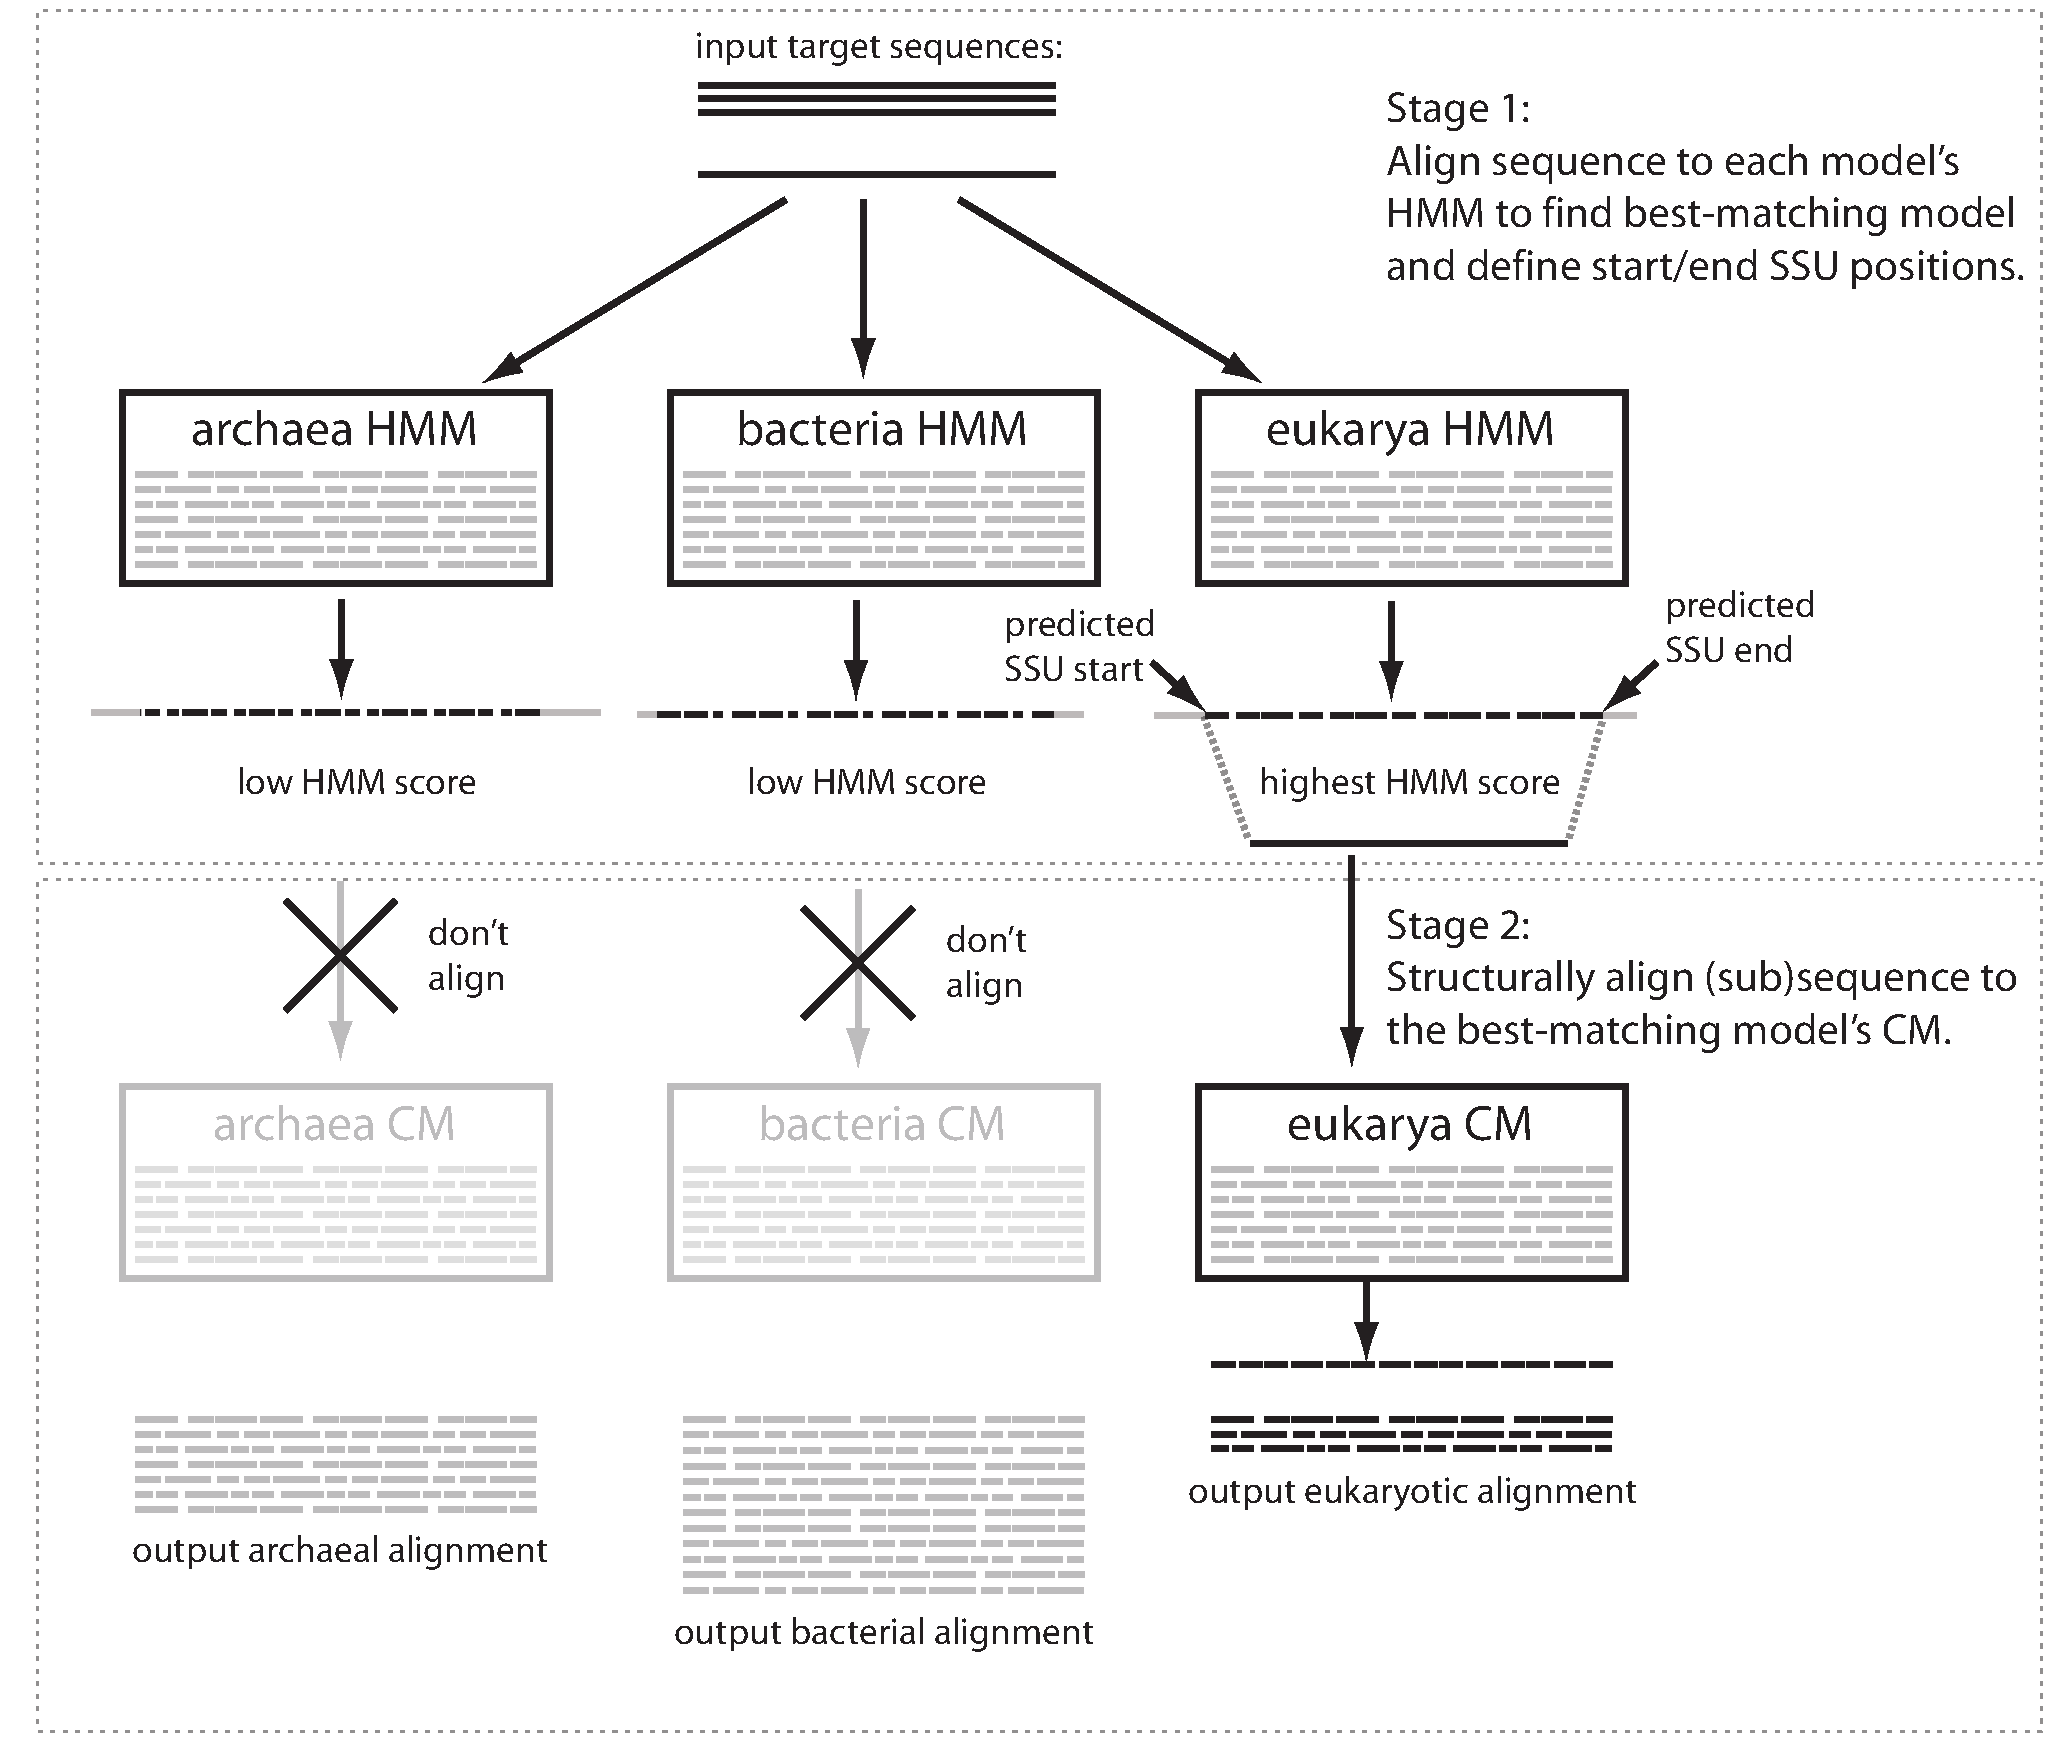
\includegraphics[width=6.5in]{Figures/ssualign-schematic}
        \caption[Schematic of the \sft{ssu-align} alignment
          pipeline]{\textbf{Schematic of the SSU-align
          alignment pipeline.} Unaligned target sequences are input to
        the program. In stage 1, each sequence is independently
        aligned using only primary sequence scoring to each of $N$
        HMMs, one built from each model in the input CM file. The
        model whose HMM alignment has the maximum bit score is the
        ``best-matching'' model for that sequence, in this example
        ``eukarya'' is the best-matching model. In stage 2, the
        unaligned (sub)sequence from the best-matching model's HMM
        alignment (potentially with some sequence trimmed off the
        ends) is aligned to the best-matching model's CM which scores
        both sequence and conserved secondary structure. The CM
        aligned target sequence is added to that model's output
        alignment. After all target sequences are processed, the
        program has output up to $N$ new structural alignments, one
        for each model that was the best-matching model for at least 1
        target sequence.}
  \end{center}
\label{fig:ssualign}
\end{figure}

\sft{ssu-align} includes the {\tt esl-alimanip} program that can
generate masks for the alignments it creates based on the posterior
probabilities for each residue in the alignment. These masks can then
be used to remove ambiguously aligned columns of the alignment prior
to using phylogenetic inference tools. %A program for creating
%secondary structure diagrams that display alignment summary statistics
%or individual sequences is also included.  
A User's Guide is supplied with \sft{ssu-align} that
explains how to use the program for creating and masking alignments.
% masking them and drawing secondary structure diagrams.

\subsection{Automated probabilistic alignment masking}

The goal of masking is to identify and remove columns containing
residues that are ambiguously aligned and therefore likely to contain
errors prior to using the alignment for phylogenetic inference.  Two
commonly used SSU masks were determined manually by David Lane and
Phil Hugenholtz (Figures 7.5 and 7.6 of \cite{Nawrocki09b}) based on
expert knowledge and extensive experience with SSU alignments.
Alignment posterior probabilities from
probabilistic models offer an alternative, objective way of evaluating
alignment ambiguity (high posterior probability means low ambiguity
and vice versa) and creating masks for any alignment.

%This is in the thesis, but it is irrelevant here.
\begin{comment}
The HMM banded alignment technique described in Chapter 8 of
\cite{Nawrocki09b} exploits
posterior probabilities calculated from the Forward and Backward
algorithms in HMM alignments. Inside and Outside, the
SCFG analogs of the Forward and Backward, can be used to calculate
posterior probabilities for CM alignment \cite{Durbin98}. These
algorithms were not implemented in \sft{infernal} prior to this work
because they are about two-fold slower than the (already slow) CYK
algorithm and because the Myers-Miller linear memory trick that made
CM SSU alignment practical (requiring 60 Mb instead of 20 Gb of RAM)
had only been applied to CYK \cite{Eddy02b}. HMM banding drastically
reduces the memory requirement for CM alignment, because only DP cells
within the bands need be allocated, making it possible to run Inside
and Outside on SSU.
\end{comment}

\subsubsection{Alignment ambiguity and length heterogeneity}

Alignment ambiguity often arises in regions of alignments with low
sequence conservation where insertions and deletions are common,
corresponding to regions of the molecule that exhibit high length
heterogeneity across different species. In such cases, it is often
difficult to determine the correct alignment because alternative
alignments seem plausible. Take for example the CM alignment
of the {\tt GUAU} subsequence of the \emph{Desulfovibrio
desulfuricans} SSU sequence to a loop region depicted in
Figure~\ref{fig:ambiguity}. The reference (consensus) sequence for the
loop ({\tt AUUCAAC}) differs from {\tt GUAU} in both sequence and
length. Consequently, the CM alignment for this loop is not well
defined, and two alternative alignments are given posterior
probabilities above $0.35$.  In contrast, the surrounding helix
region, for which higher sequence similarity exists between the two
sequences, is aligned confidently with high posterior probabilities.

\begin{figure}
\ttfamily
\footnotesize
\begin{center}
%ORIGINAL DATA is from Macbook: 
%/Users/nawrockie/school/notebook/9_0309_ths/latex/ssu/ambiguity_example
\begin{tabular}{ll}
00904::Desulfovibrio\_desulfuricans-1 &                             GAUGUCGGGGA--GUAU---UCUUCGGUGUC \\
\#=GR 00904::Desulfovibrio\_desulfuricans-1 POSTX. &                99999999999--5665---89999999999 \\
\#=GR 00904::Desulfovibrio\_desulfuricans-1 POST.X &                99999999996--8009---79999999999 \\
& \\
00904::Desulfovibrio\_desulfuricans-2              &                GAUGUCGGGGA---GUAU--UCUUCGGUGUC \\
\#=GR 00904::Desulfovibrio\_desulfuricans-2 POSTX. &                99999999999---3333--89999999999 \\
\#=GR 00904::Desulfovibrio\_desulfuricans-2 POST.X &                99999999996---6665--79999999999 \\
& \\
\#=GC SS\_cons                        &                             <<<<<<<<<<<<.......>>>>>>>>>>>> \\
\#=GC RF                              &                             GGUGUuGGgggcAuUcaACgcccUCaGUGCC \\
\end{tabular}
\rmfamily

\vspace{0.2in}
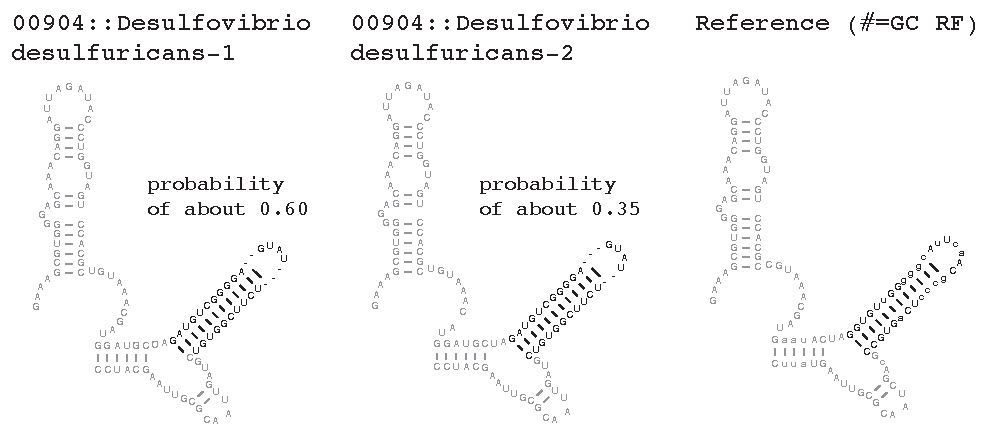
\includegraphics[width=5.7in]{Figures/ambiguity}

\caption[Example of alignment ambiguity in a hairpin loop.]{
  \textbf{Example of alignment ambiguity in a hairpin loop.}  Top: A
  alignment fragment of two different alignments of the
  \emph{Desulfovibrio desulfuricans} (sequence accession
  \texttt{M34113}) sequence from the \sft{ssu-align} bacterial seed
  alignment for the region between consensus columns $861$ and $881$.
  Each alignment is annotated with its posterior probability in the
  \texttt{\#=GR POSTX.} and \texttt{\#=GR POST.X} rows.  For example,
  the second \texttt{A} in the first aligned sequence has a posterior
  probability of $0.60$ of being aligned in its current position. The
  probability this \texttt{A} aligns in the next position over, as it
  does in the second alignment, is $0.36$.  The \texttt{\#=GC
    SS\_cons} and \texttt{\#=GC RF} rows correspond to the consensus
  secondary structure and sequence respectively.  The alignments were
  created using \texttt{cmalign} to align this sequence to the
  bacterial CM with the \texttt{--sample} option.  Bottom: The
  secondary structures corresponding to the two possible alignments of
  the \emph{D. desulfuricans} and the reference alignment.  Residues
  in the actual alignment are black. Residues surrounding the
  alignment fragment are gray.}
\end{center}
\label{fig:ambiguity}
\end{figure}

\subsubsection{Inserted columns should always be excluded during masking}

Importantly, any CM alignment mask should automatically exclude 
every insert column of the alignment. This is because profile
probabilistic models like CMs do not actually align inserted residues
(residues aligning to insert states) between different sequences, but
rather simply insert them between the appropriate consensus columns in
the alignment. This means that sequence residues appearing in the same
insert alignment columns are not aligned with respect to each
other and consequently should be removed prior to phylogenetic
analysis which assumes aligned residues are homologous.
%An example of inserted residues that are obviously not correctly
%aligned is shown in Figure~\ref{fig:inserts}.

\subsubsection{Benchmarking probabilistic masking}

I decided on a simple method for defining masks that requires that
a given fraction $x$ of the residues in an aligned consensus
(non-insert) column have a posterior probability above a minimum
threshold $y$ to be included (not pruned away) by the mask. I tested
%both of these approaches on
this approach with different $x$ and $y$ values on 
the SSU alignment test from the Kolbe09 benchmark \cite{KolbeEddy09}
described in Chapter 8 of \cite{Nawrocki09b}. Briefly, the test consists of building a CM
from an aligned subset of $101$ training sequences from a \emph{gold
standard} \db{crw} alignment and aligning a separate subset of $51$ test
sequences, where the training and testing sets have been defined such
that no train/test pair is more than 80\% identical. Accuracy is
measured by the similarity of the CM alignment of test sequences to
the original \db{crw} alignment (for more details, see Chapter 8 of
\cite{Nawrocki09b} or
\cite{KolbeEddy09}). The purposefully low sequence similarity between
the training and test set sequences are meant to increase the
difficulty of the benchmark. 

The effect of masking using several different combinations of $x$ and
$y$ values on the alignment accuracy and coverage of CM alignment on
the Kolbe09 benchmark is summarized in
Table~\ref{tbl:kolbe09-pp}. Coverage is defined as the fraction of
residues in the test alignment that are included by the mask. Accuracy
is the fraction of residues included by the mask which are correctly
aligned (as defined in Chapter 8 of \cite{Nawrocki09b} and \cite{KolbeEddy09}. 
The results indicate a trade-off between 
coverage and accuracy: coverage decreases but accuracy increases
as $x$ and $y$ increase, because the mask becomes more stringent,
requiring a larger fraction of more confidently aligned residues in
included columns. There is no clear best-performing combination of $x$
and $y$. \sft{ssu-align} uses $0.95$ for both $x$ and $y$ as the
default, a strategy which attains $99.74\%$ accuracy and $85.37\%$
coverage on the benchmark. 

% original data from:
%latex/submit-tobesubmitted/pp-ssualign-tables/pp-table.txt
%                   800              850              900              925              950              975              990  
%y: 800    0.9576/0.9897    0.9538/0.9903    0.9367/0.9928    0.9297/0.9935    0.9253/0.9939    0.9088/0.9949    0.9014/0.9952  
%y: 850    0.9393/0.9921    0.9294/0.9933    0.9214/0.9942    0.9147/0.9946    0.9109/0.9949    0.8949/0.9953    0.8848/0.9958  
%y: 900    0.9186/0.9946    0.9155/0.9948    0.9095/0.9950    0.9008/0.9955    0.8940/0.9959    0.8774/0.9965    0.8634/0.9971  
%y: 925    0.9111/0.9950    0.9008/0.9956    0.8869/0.9961    0.8797/0.9963    0.8724/0.9968    0.8533/0.9973    0.8441/0.9975  
%y: 950    0.8987/0.9958    0.8811/0.9966    0.8691/0.9969    0.8599/0.9972    0.8537/0.9974    0.8396/0.9977    0.8214/0.9978  
%y: 975    0.8626/0.9972    0.8499/0.9976    0.8404/0.9977    0.8354/0.9979    0.8234/0.9981    0.7954/0.9982    0.7740/0.9985  
%y: 990    0.7720/0.9981    0.7586/0.9983    0.7424/0.9985    0.7209/0.9986    0.6904/0.9988    0.6420/0.9990    0.5969/0.9990  
%
% without 85%
%                   800              900              925              950              975              990  
%y: 800    0.9576/0.9897    0.9367/0.9928    0.9297/0.9935    0.9253/0.9939    0.9088/0.9949    0.9014/0.9952  
%y: 900    0.9186/0.9946    0.9095/0.9950    0.9008/0.9955    0.8940/0.9959    0.8774/0.9965    0.8634/0.9971  
%y: 925    0.9111/0.9950    0.8869/0.9961    0.8797/0.9963    0.8724/0.9968    0.8533/0.9973    0.8441/0.9975  
%y: 950    0.8987/0.9958    0.8691/0.9969    0.8599/0.9972    0.8537/0.9974    0.8396/0.9977    0.8214/0.9978  
%y: 975    0.8626/0.9972    0.8404/0.9977    0.8354/0.9979    0.8234/0.9981    0.7954/0.9982    0.7740/0.9985  
%y: 990    0.7720/0.9981    0.7424/0.9985    0.7209/0.9986    0.6904/0.9988    0.6420/0.9990    0.5969/0.9990  

%\begin{sidewaystable}
\begin{table}
\scriptsize
\begin{center}
\begin{tabular}{|c||cc|cc|cc|cc|cc|cc|}
\multicolumn{1}{c}{} & \multicolumn{12}{c}{$x$ (fraction of sequences with posterior probability above y)} \\ \hline
      & \multicolumn{2}{c|}{0.800} & \multicolumn{2}{c|}{0.900} & \multicolumn{2}{c|}{0.925} & \multicolumn{2}{c|}{0.950} & \multicolumn{2}{c|}{0.975} & \multicolumn{2}{c|}{0.990} \\ \cline{2-13}
 $y$  &     cov  & acc    &  cov    & acc     &  cov    & acc    &  cov    & acc    &     cov & acc    &      cov & acc    \\ \hline
& & & & & & & & & & & & \\
0.800 &   0.9576 & 0.9897 &  0.9367 & 0.9928  &  0.9297 & 0.9935 &  0.9253 & 0.9939 &  0.9088 & 0.9949 &   0.9014 & 0.9952 \\
& & & & & & & & & & & & \\
0.900 &   0.9186 & 0.9946 &  0.9095 & 0.9950  &  0.9008 & 0.9955 &  0.8940 & 0.9959 &  0.8774 & 0.9965 &   0.8634 & 0.9971 \\
& & & & & & & & & & & & \\
0.925 &   0.9111 & 0.9950 &  0.8869 & 0.9961  &  0.8797 & 0.9963 &  0.8724 & 0.9968 &  0.8533 & 0.9973 &   0.8441 & 0.9975 \\
& & & & & & & & & & & & \\
0.950 &   0.8987 & 0.9958 &  0.8691 & 0.9969  &  0.8599 & 0.9972 &  {\bf 0.8537} & {\bf 0.9974} &  0.8396 & 0.9977 &   0.8214 & 0.9978 \\
& & & & & & & & & & & & \\
0.975 &   0.8626 & 0.9972 &  0.8404 & 0.9977  &  0.8354 & 0.9979 &  0.8234 & 0.9981 &  0.7954 & 0.9982 &   0.7740 & 0.9985 \\
& & & & & & & & & & & & \\
0.990 &   0.7720 & 0.9981 &  0.7424 & 0.9985  &  0.7209 & 0.9986 &  0.6904 & 0.9988 &  0.6420 & 0.9990 &   0.5969 & 0.9990 \\ \hline
\end{tabular}
\end{center}
\caption[Effect of different masking strategies on CM alignment
  accuracy and coverage on the Kolbe09 SSU alignment benchmark]{
  \textbf{Effect of different masking strategies on CM alignment
  accuracy and coverage on the Kolbe09 SSU alignment benchmark.}
  Alignments were performed using \sft{infernal} 1.01's {\tt cmalign}
  program with the {\tt --cyk} flag, which performs HMM banded CYK
  alignment with $\tau=10^{-7}$. Masks were defined as follows: any
  consensus alignment column in which more than $x$ fraction of the
  aligned residues have a posterior probability of at least $y$ is
  included by the mask. All other columns are excluded (not
  counted). ``cov'' (coverage) is the fraction of residues in the test
  alignment that are included by the mask. ``acc'' (accuracy) is the
  fraction of residues included by the mask which are correctly
  aligned. The values cooresponding to the \sft{ssu-align} default
  banding strategy $x=0.95$ and $y=0.95$ are in bold-faced type.  The
  Kolbe09 benchmark and its definition of alignment correctness are
  described in more detail in Chapter 8 of \cite{Nawrocki09b} and in
  \cite{KolbeEddy09}. Masks were computed with the {\tt esl-alimanip}
  program with flags {\tt --p-rf --p-fract <x> --p-thresh <y>}.}
\label{tbl:kolbe09-pp}
\end{table}
%\end{sidewaystable}

A separate validation of the automated masking strategy, apart from
benchmarking is via comparison to the manually created masks of David
Lane and Phil Hugenholtz discussed in Chapter 7 of \cite{Nawrocki09b}. To
enable the comparison, I used the \sft{ssu-align} bacterial CM to
realign each of the bacterial seed sequences and masked the resulting
alignment based on posterior probabilities using $x$ and $y$ values of
$0.95$. The resulting mask overlaid on the \sft{ssu-align} bacterial
consensus secondary structure model is shown next to David Lane's mask
on the \emph{E. coli} SSU structure in Figure~\ref{fig:infvlane}. In
general, the same regions are excluded by both masks. The
\sft{ssu-align} mask excludes significantly fewer positions than does
the Lane mask.  This is to be expected and does not suggest the
\sft{ssu-align} is in any way ``better'' than the Lane mask.  The
\sft{ssu-align} mask was derived from an alignment consisting only of
the seed sequences the model was parameterized from, which the model should
be able to align with high confidence. The key point here is that the
\sft{ssu-align} mask is different from the Lane mask because it is specific to the
alignment it was created for. The ability to automatically construct 
alignment specific masks is an important feature of \sft{ssu-align} that
distinguishes it from other alignment tools. 

\begin{sidewaysfigure}
  \begin{center}
    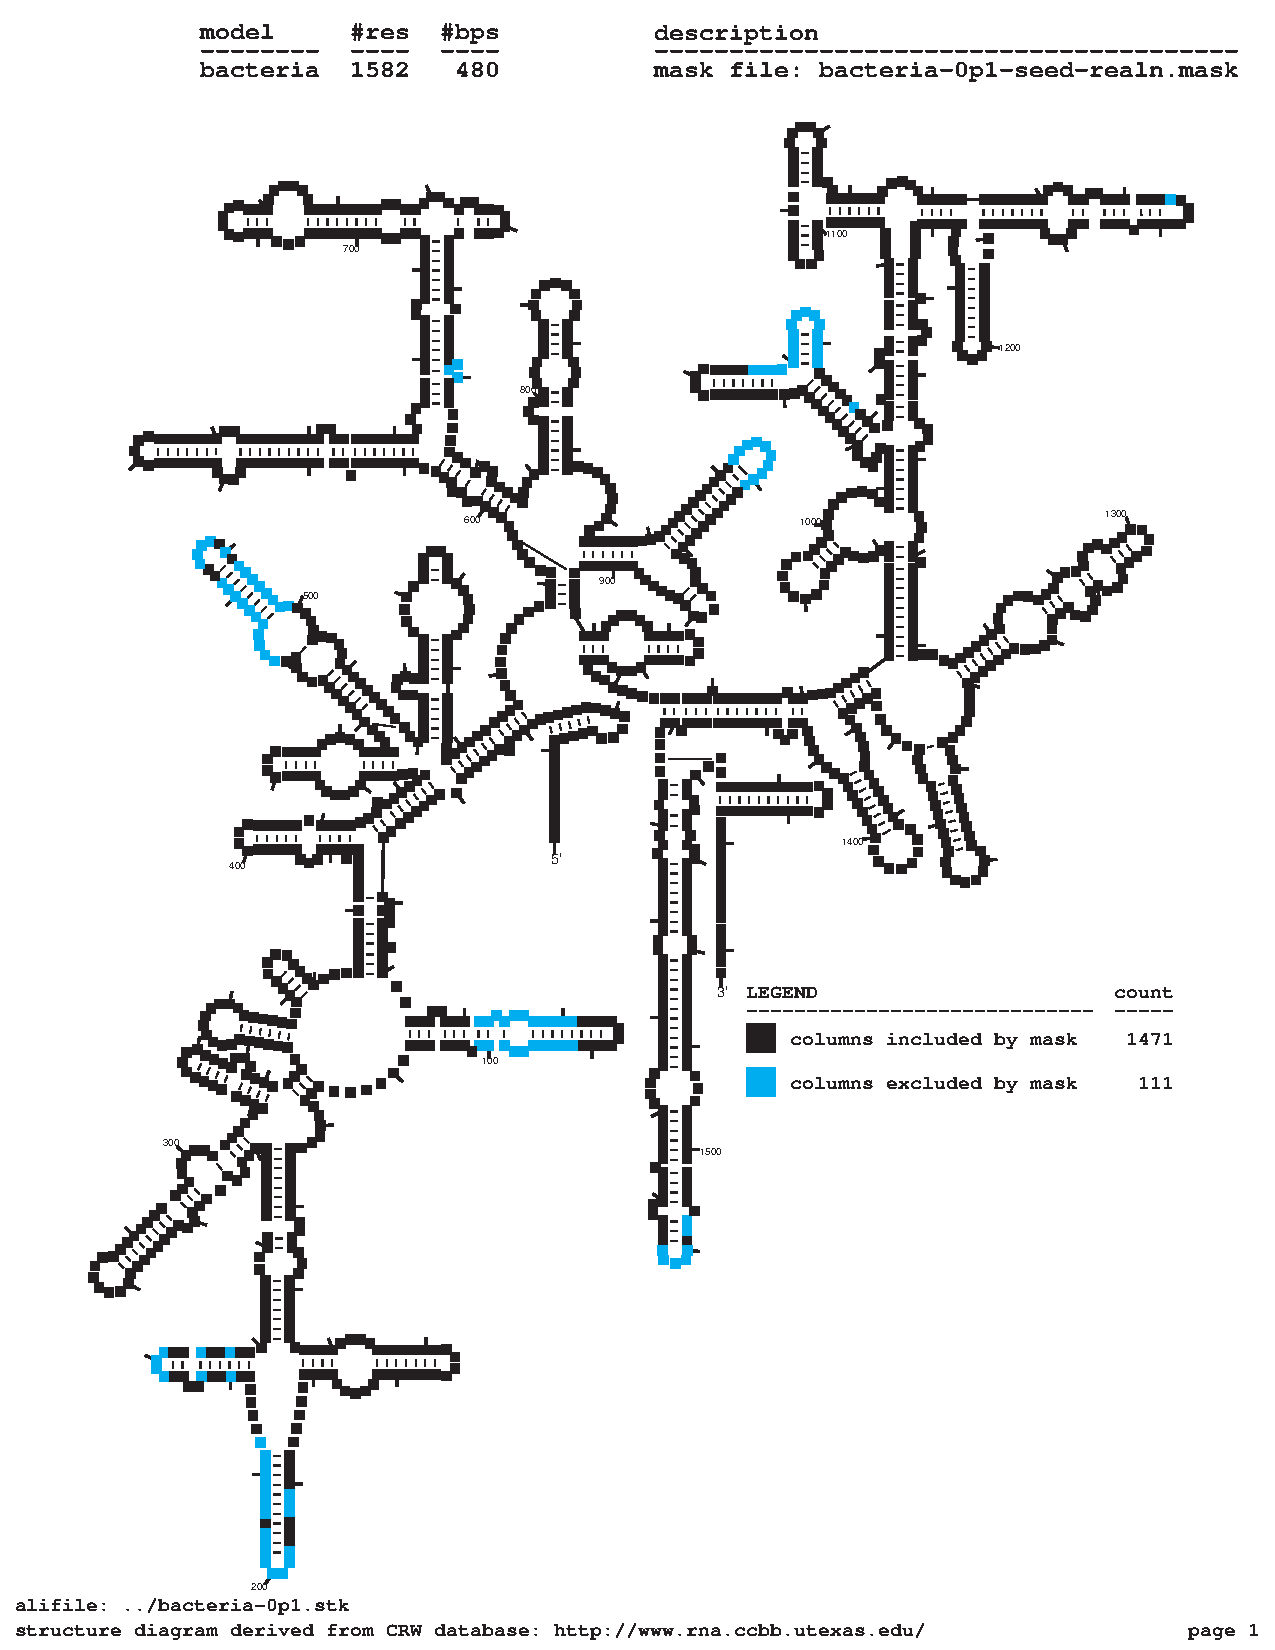
\includegraphics[width=3.7in]{Figures/bacteria-0p1-maskcol}
    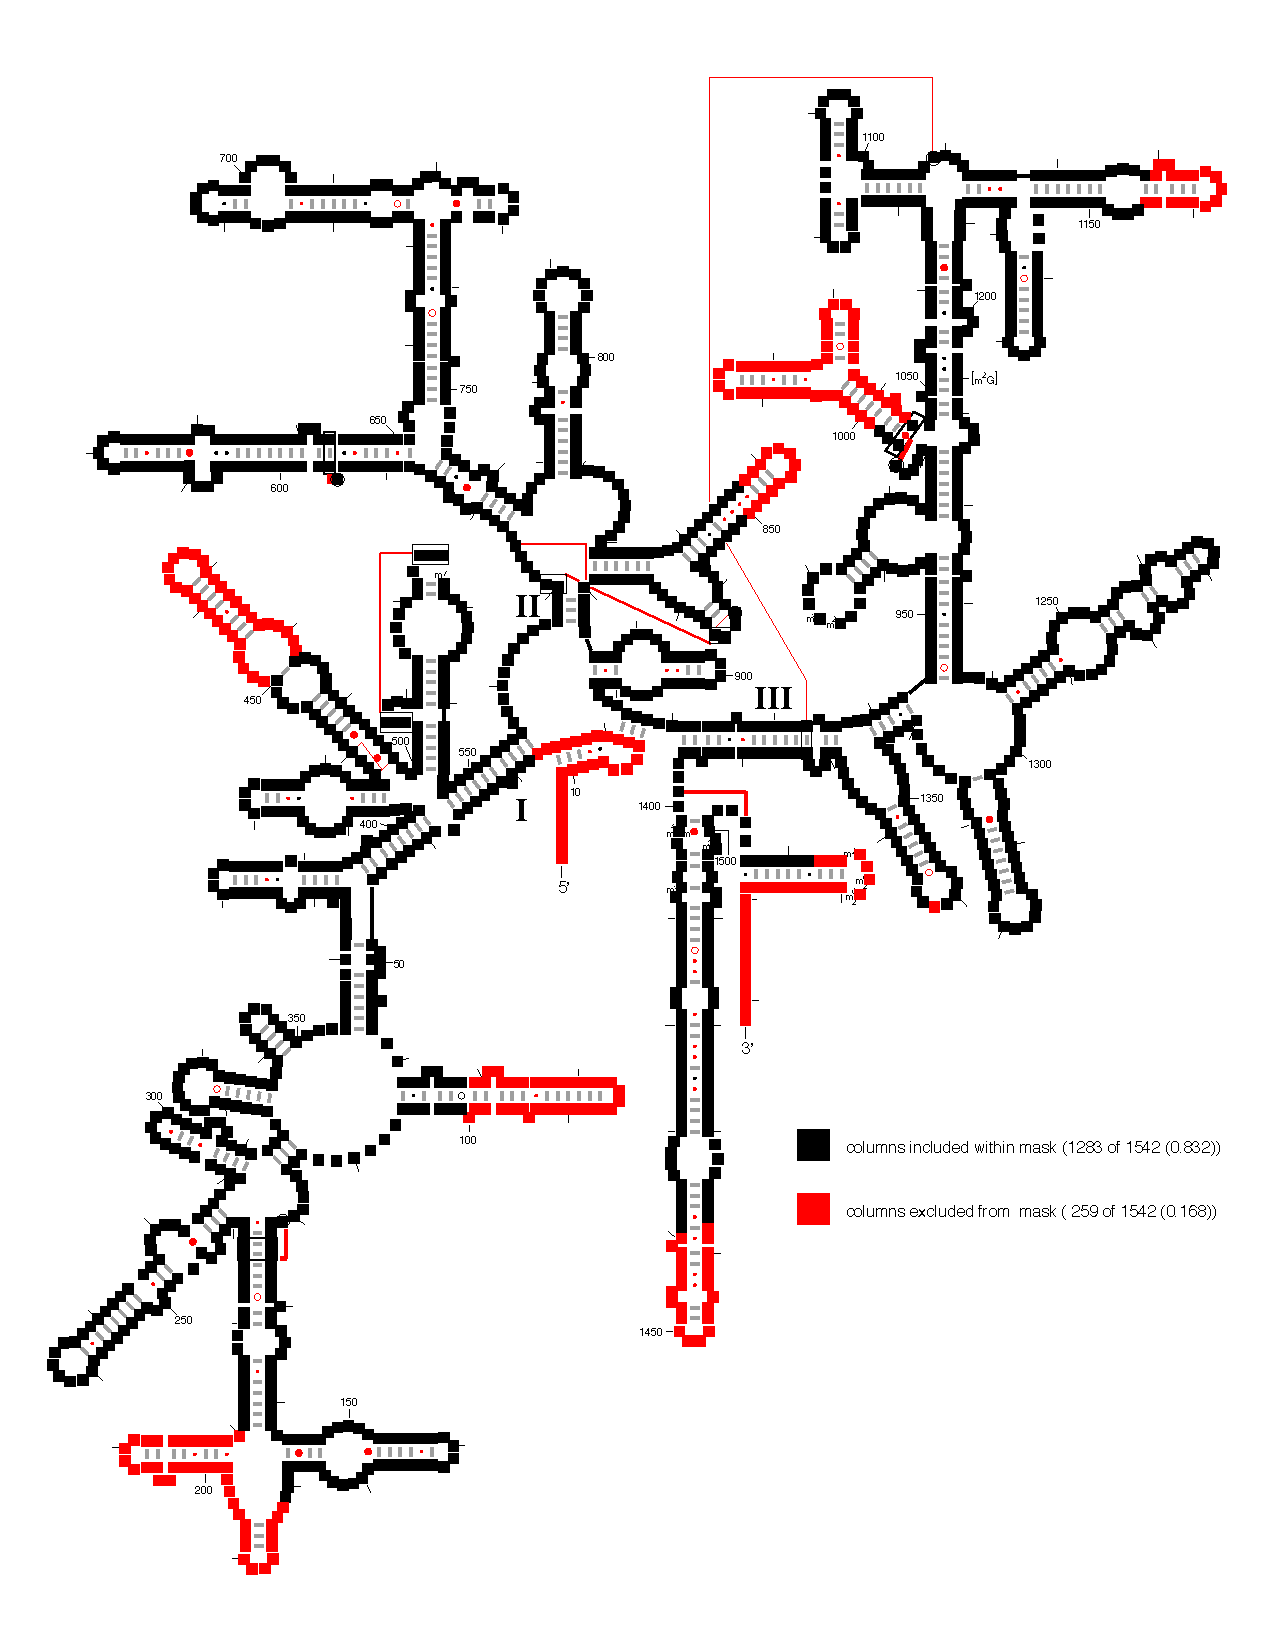
\includegraphics[width=3.7in]{Figures/lane-ecoli}
  \end{center}
  \caption[Similarity of an \sft{ssu-align} automatically
    constructed mask with David Lane's SSU alignment mask.]{
    \textbf{Similarity of an \sft{ssu-align} automatically
      constructed mask (left) with David Lane's SSU alignment mask (right).
    \emph{Escherichia coli}}. Black columns are included by
  the mask for phylogenetic analyses. Blue (left) or red (right) columns are excluded
  by the mask for phylogenetic analyses. 
  The \sft{ssu-align} mask was derived automatically based on a
    realignment of the bacterial seed sequences as explained in the
    text. The right diagram was derived from the overlay of the ``LMPH'' mask on the
  \db{greengenes} database's \emph{Core Set} alignment of the
  \emph{E. coli} sequence (\db{GenBank} accession J01695). Both diagrams
    were generated with the {\tt esl-ssudraw} program included 
    with \sft{ssu-align}.}
\label{fig:infvlane}
\end{sidewaysfigure}

The automatically masked bacterial alignment nicely 
demonstrates the tight relationship between length heterogeneity
and alignment ambiguity as measured by posterior probabilities. 
The positions excluded from the mask are tightly
correlated with positions of the alignment that include at least some
gaps (deletions) in consensus positions corresponding to length
heterogeneity between different sequences. The effect can be seen
clearly in Figure~\ref{fig:bacdelmask} which displays the frequency of
deletions of each consensus column on a secondary structure diagram of
SSU. Positions excluded from the automated mask appear as open
circles. Note that the circles occur in clusters that are almost
always adjacent to a region with at least a few deletions. 

\begin{figure}
\begin{center}
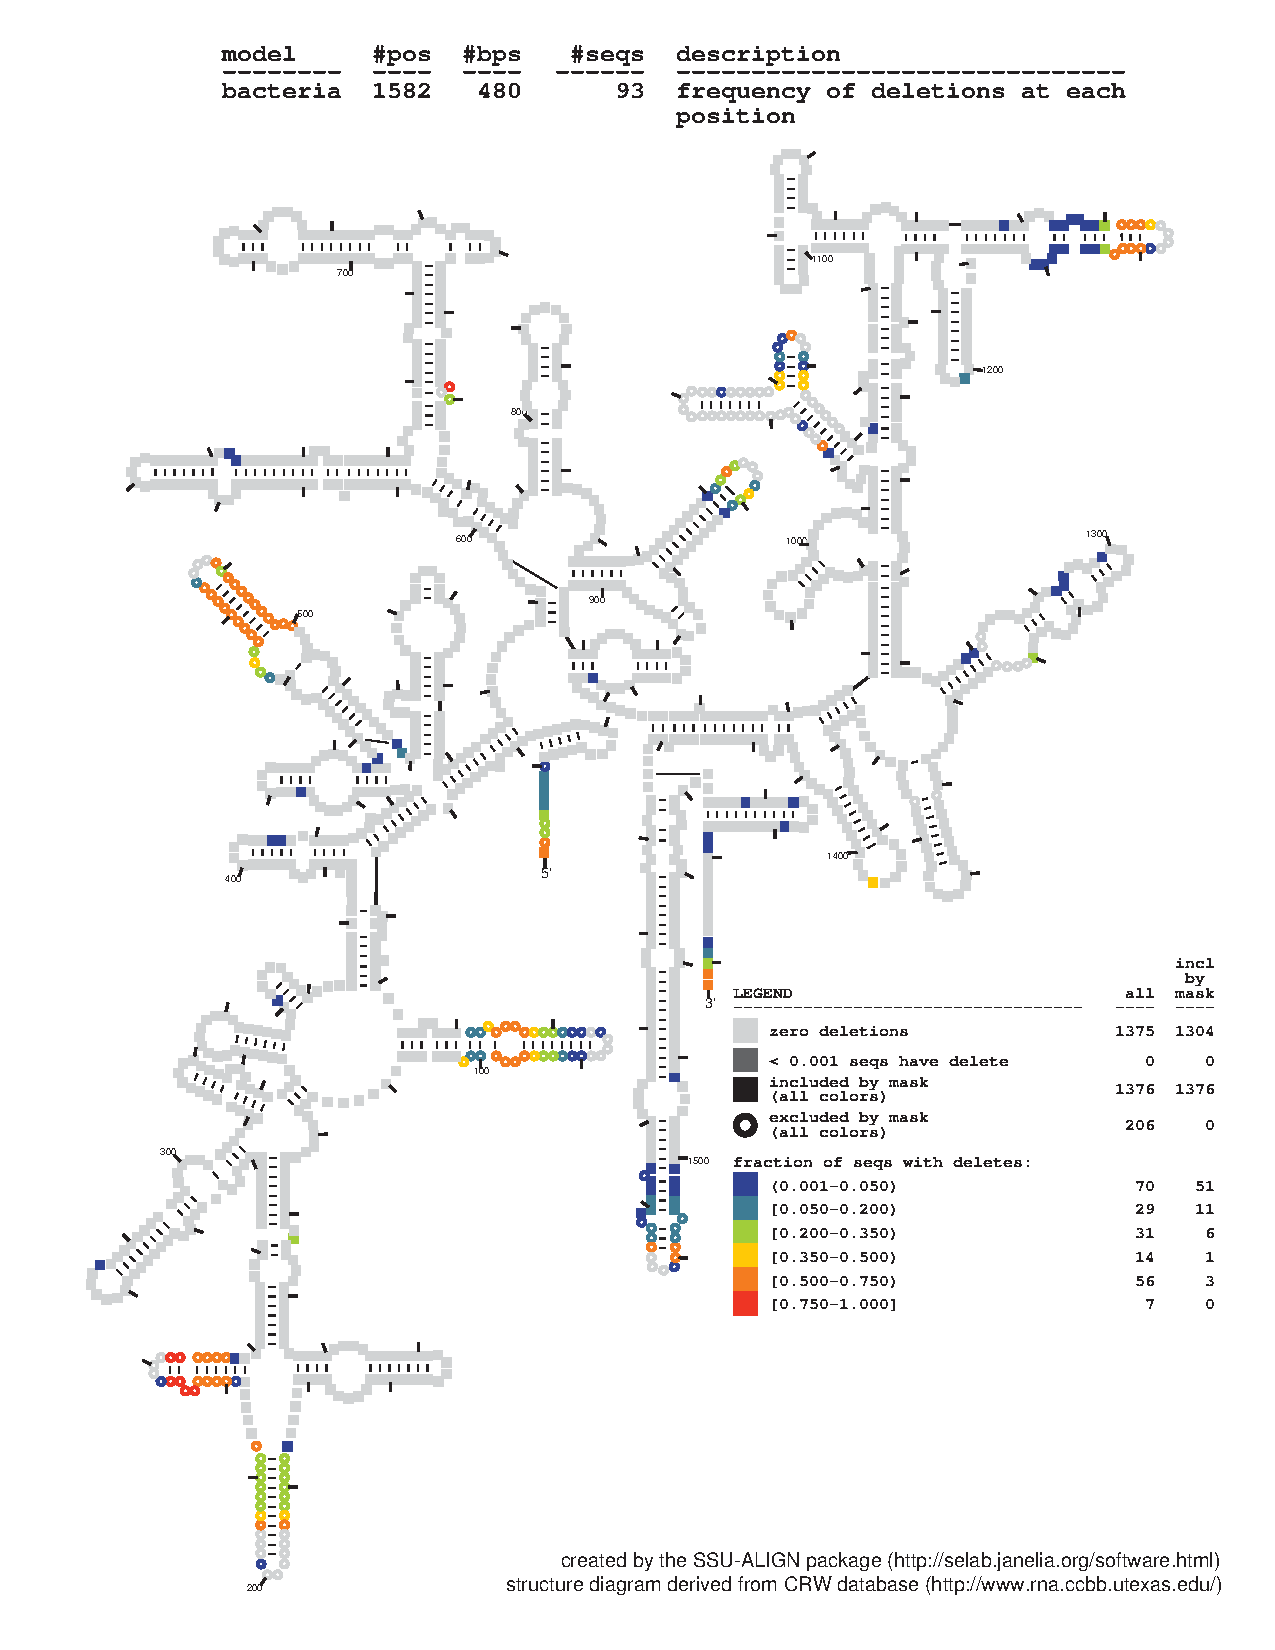
\includegraphics[width=5.7in]{Figures/bacteria-0p1-dall-wmask}
\end{center}
\caption[Secondary structure diagram displaying frequency of deletions
  of each consensus position in a masked bacterial alignment of the SSU seed
  sequences]{\textbf{Secondary structure diagram displaying frequency of deletions
  of each consensus position in a masked bacterial alignment of the SSU seed
  sequences.} Statistics correspond to a CM alignment of the bacterial
  seed sequences using the \sft{ssu-align} bacterial CM. Consensus positions
  excluded from the mask (denoted as circles) are those for which 
  more than 5\% of the residues have a posterior probability below
  $0.95$, as explained in the text. This diagram was generated by the
  {\tt esl-ssudraw} program included in \sft{ssu-align}.}
\label{fig:bacdelmask}
\end{figure}

\subsection{Implementation}

\sft{ssu-align} is itself a \sft{perl} script that orchestrates the
use of the \sft{infernal} software package's \texttt{cmsearch} and
\texttt{cmalign} programs \cite{infernal} and Sean Eddy's \sft{easel}
sequence analysis library's \texttt{esl-sfetch} (\sft{easel} is
included in \sft{infernal}).  The input CM file must have been created
prior to running \sft{ssu-align}, by \sft{infernal}'s \texttt{cmbuild}
program. An SSU CM file is provided with the program, but users can
also build their own. Stage 1 HMM scoring is performed by
\texttt{cmsearch}. Sequence truncation, when necessary, is performed
by \texttt{esl-sfetch}. Stage 2 CM alignment of targets to their
best-matching models is performed by \texttt{cmalign}. Alignment
masking is performed by \sft{easel}'s \texttt{esl-alimanip} program. 
%Finally, structure diagrams are created by
%\sft{easel}'s \texttt{esl-ssudraw} program.
%I will now explain each step in more detail.

\subsection{SSU-align's SSU rRNA sequence and structure models}

CMs model both the conserved sequence and secondary structure of an
RNA family. Constructing CMs requires as input a multiple sequence
alignment with well-nested consensus secondary structure
annotation. An important question in the design of the \sft{ssu-align}
program was where to obtain these alignments from. I decided to use
the \db{Comparative RNA Website} (\db{CRW}) \cite{CannoneGutell02} as
the source because it has the largest amount of high quality
structural data of any of the SSU databases (see
Chapter 7 of \cite{Nawrocki09b}).

The structure models used by \db{crw} are based on nearly thirty years of
comparative analysis. The first secondary structures of SSU were
created in the early 1980s, by Carl Woese, Harry Noller, Robin Gutell
and others using comparative sequence analysis to identify covarying
positions indicative of structural relationships such as base-pairs
\cite{Woese80,Noller81,Woese83}. Since then, Gutell and his
colleagues have continued to refine those models. Their comparative
approach was validated in 2000, when the crystal structure of the
small subunit of \emph{Thermus thermophilus} was solved
\cite{Wimberly00} and 97\% of the predicted base-pairs in the then
current bacterial secondary structure model were confirmed
\cite{Gutell02}.

Over the past twenty years, Gutell and coworkers have constructed SSU
alignments of thousands of sequences using a combination of automated
techniques and manual curation. As part of this process, they have
singled out novel (phylogenetically distinct) SSU sequences and
manually predicted their secondary structures. The alignment and
structural data is publicly available in the \db{crw} database
\cite{CannoneGutell02}. 

\subsubsection{SSU secondary structure data from the Comparative RNA
  Website} 

\db{CRW} includes separate SSU alignments for archaea, bacteria,
chloroplasts, eukarya (nuclear), and mitochondria. I concentrated only
on the archaeal, bacterial, and eukaryotic alignments for the initial
version of \sft{ssu-align}.  Unfortunately, the \db{crw} alignments
are not structurally annotated, so they cannot be used directly to
build CMs. However, \db{crw} curators have predicted structures for a
subset of the sequences in each alignment.  To create structure
annotated alignments I mapped the structural data onto the alignments
through a series of steps as described below.  Statistics on the
\db{crw} alignments and structural data as of May 13, 2009 are given
below:

\begin{center}
\begin{tabular}{l|rr|r}
       & \multicolumn{2}{c|}{\# of aligned}& \\
       & \multicolumn{2}{c|}{sequences}    & \# of \\ \cline {2-3}
family & primary & seed                   & structures \\ \hline
archaea&     788 &  132                   & 25 \\
bacteria&  35998 & 1266                   & 231 \\
%chloroplast& 404 & N/A                    & 33 \\
eukarya&    1937 & N/A                    & 259 \\
%mitochondria & 899 & N/A                  & 96 \\
\end{tabular}
\end{center}

The {\em primary} alignments are the largest, most complete alignments
in \db{crw}. The {\em seed} alignments are smaller and ``highly
refined''. Because CM alignment accuracy is highly dependent on the
quality of the seed alignment used to build the model, I decided to
concentrate on the seed alignments for archaea and bacteria and the
primary alignment for the eukarya (because no eukaryotic seed exists).

In an effort to ensure high accuracy, I decided not to
use the full \db{crw} alignments as my seed alignments but rather to use
subsets of the alignments containing only the sequences for which
individual structure predictions exist.  There were two main reasons
for this. First, the sequences that were chosen for individual
structure prediction were those that represented the major
phylogenetic groups and ``reveal the major forms of sequence and
structure conservation and variation'' \cite{CannoneGutell02}. This
suggests they would constitute a good seed alignment from which to
build a profile. (A good seed alignment should be representative of
the family and generally does not benefit from redundancy
\cite{Durbin98}.) Secondly, after predicting an individual structure,
the \db{crw} curators use the structure to revise the larger alignments,
which suggests that these particular sequences are the most reliably
aligned because they received the most expert attention.

\subsubsection{Defining consensus structures from individual structures}

Obtaining the consensus structure annotated alignments needed to build
CMs required combining the individual structural data and the
alignments. One simple approach would be to define a single individual
structure $x$ as the consensus structure and impose it on the entire
alignment. However, this is not ideal because it means the consensus
\emph{will not} include structural features that are absent from $x$
but present in other individual structures, and \emph{will} include
structural features that may be unique to $x$, or at least uncommon in
other individual structures. A better approach is to combine or
average the individual structures in a reasonable way to determine the
consensus structure, and then impose it on the alignment. The
procedure I used for deriving consensus structure annotated seed
alignments from the \db{crw} data is shown in Figure~\ref{fig:crw2seed}.

\begin{figure}
  \begin{center}
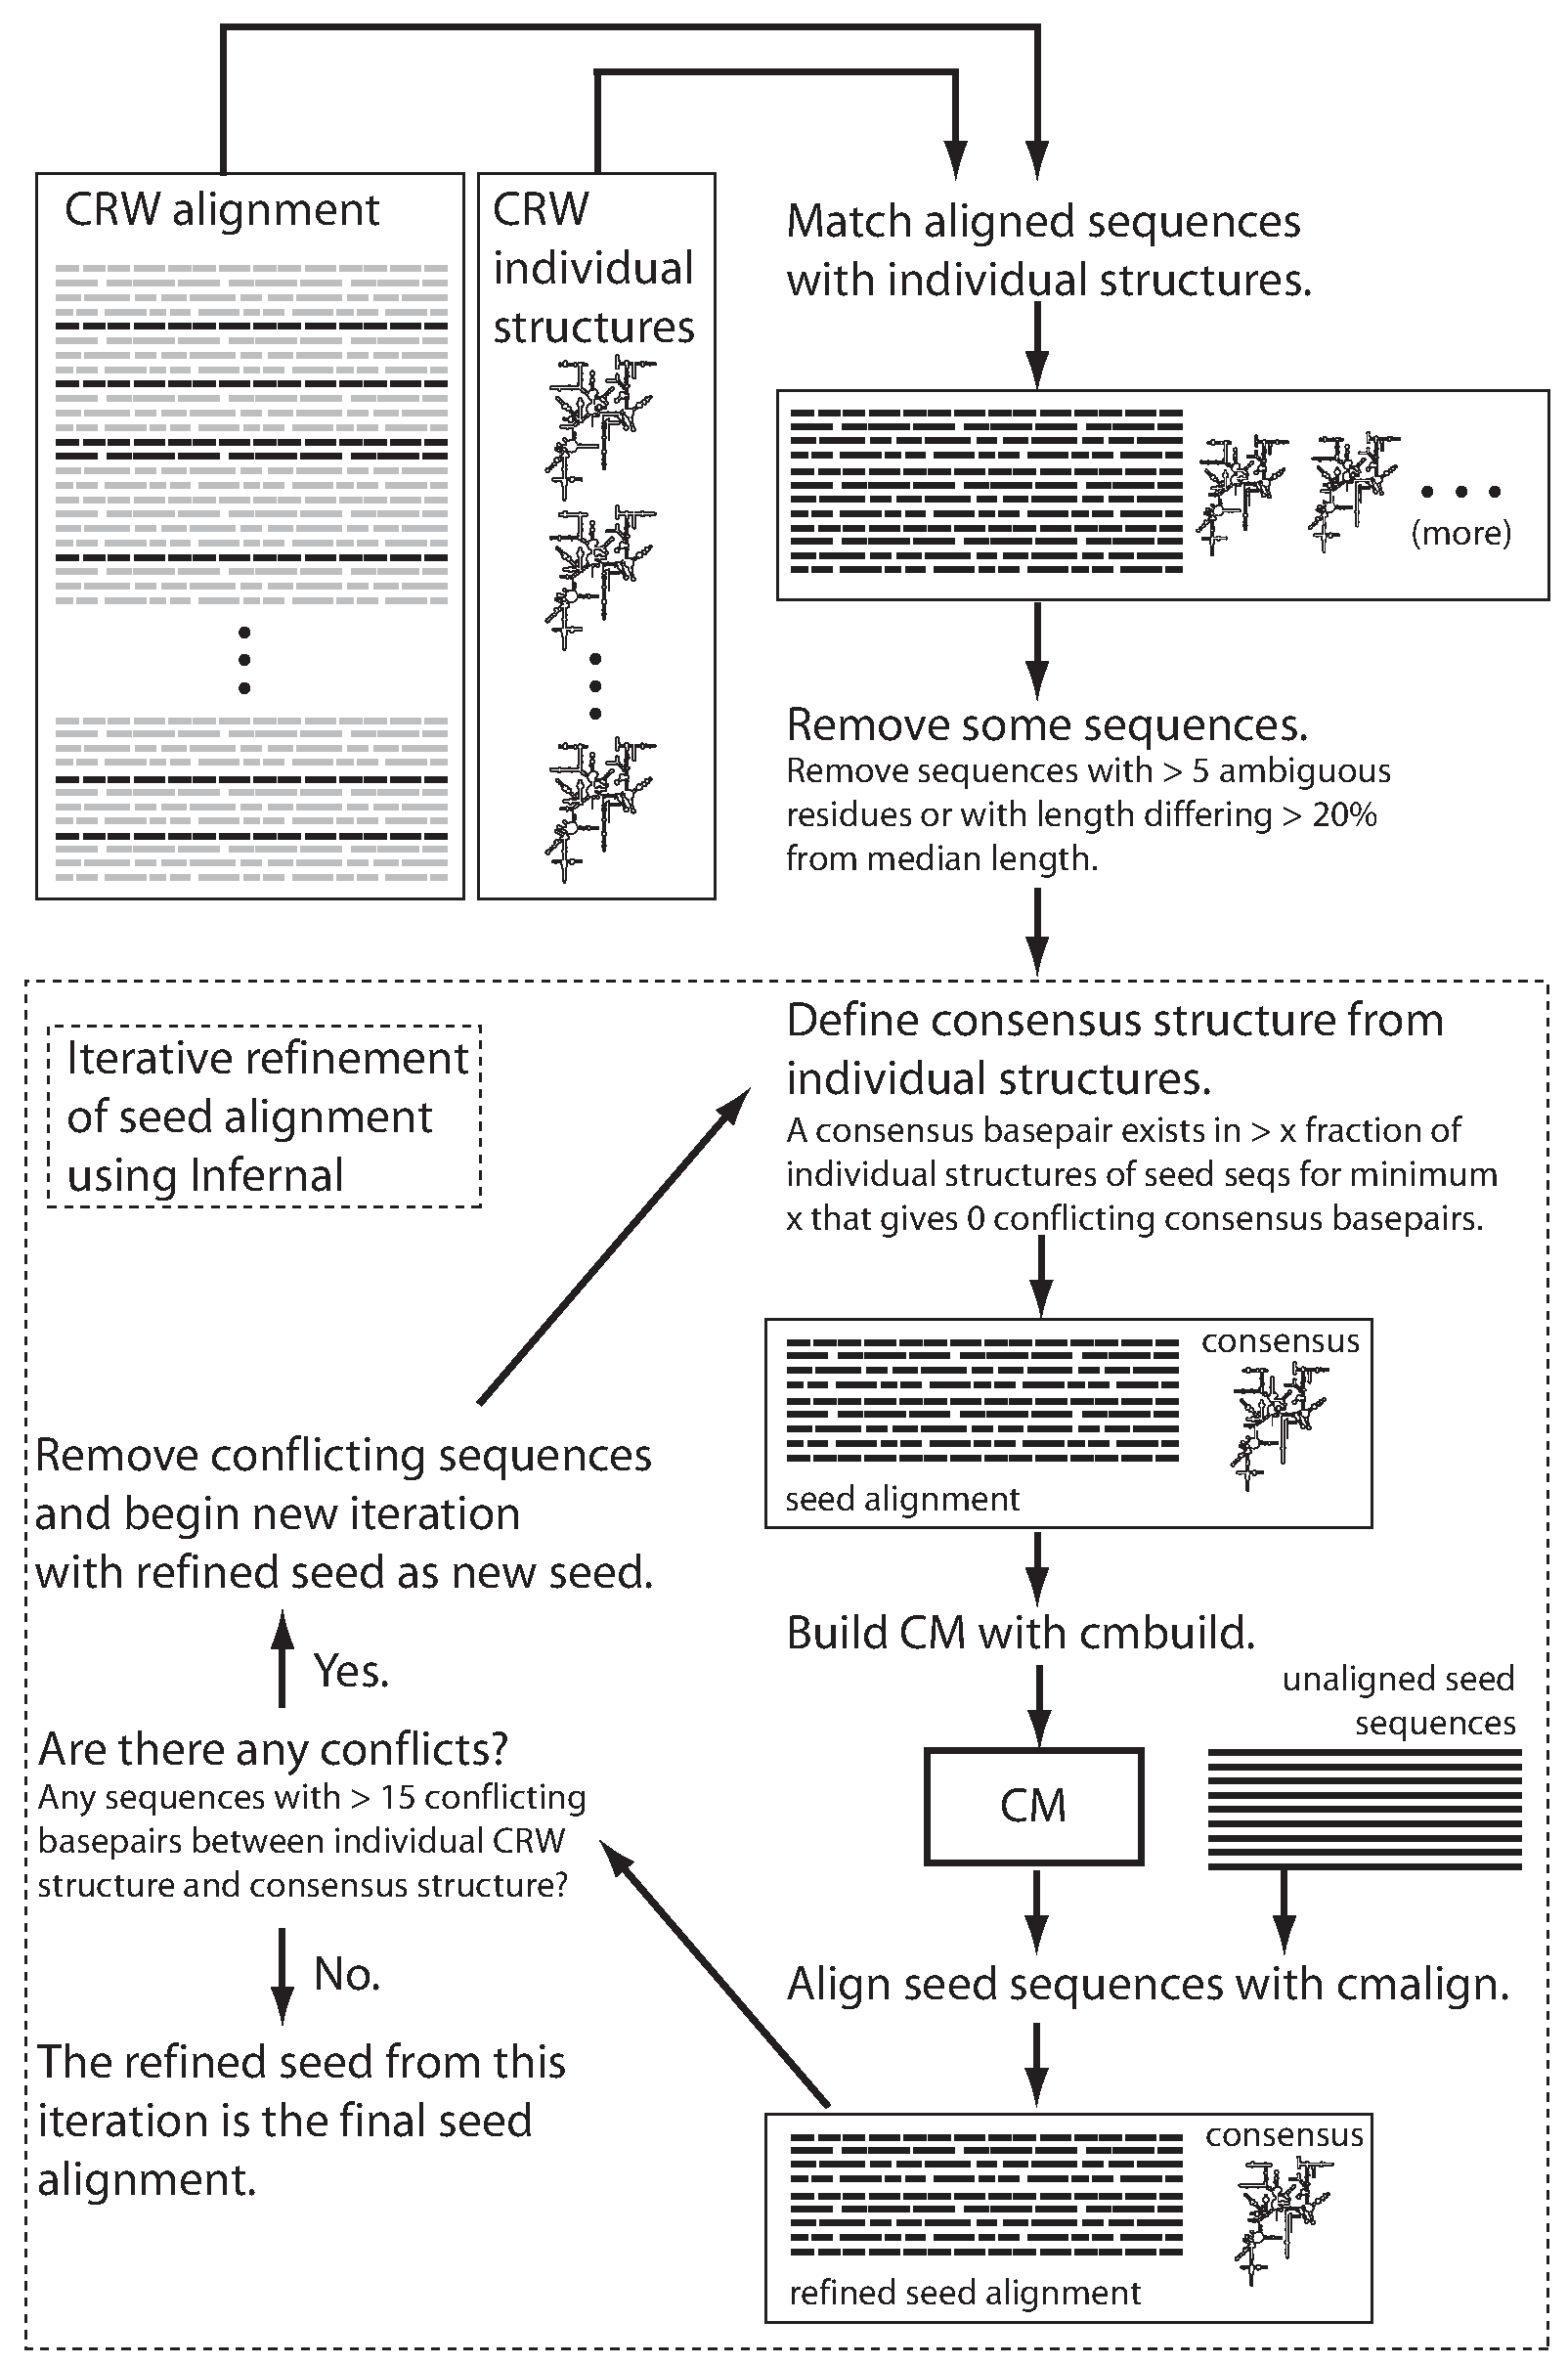
\includegraphics[height=6.9in]{Figures/crw2seed-schematic}
        \caption[The procedure for converting SSU alignments and
          individual structures from \db{crw} to seed alignments for
          \sft{ssu-align}.]  {\textbf{The procedure for converting
            SSU alignments and individual structures from \db{crw} to seed
            alignments for \sft{ssu-align}}. \db{crw} individual structures
          only exist for a small subset of the sequences from the \db{crw}
          alignments (the black sequences among the majority of gray
          ones). Each conversion step is explained
          in more detail in the text. 
          Figure~\ref{fig:conflict}
          demonstrates an example of conflicting base-pairs. 
          Table~\ref{tbl:crw2seed} includes alignment
          statistics and number of sequences surviving each step for
          each of the three seed alignments derived from \db{crw}.}
  \end{center}
\label{fig:crw2seed}
\end{figure}

The first step was to extract the aligned sequences that matched to
the individual structures from the master alignments.  An individual
structure sequence $i$ and an aligned sequence $a$ qualified as match
if: $a$ and $i$ both had the same sequence accession, and the
unaligned sequence of $a$ was either identical to $i$ or an exact
subsequence of $i$.  Not all of the individual structures $i$ had a
matching aligned sequence $a$ per these criteria.  The number of
matches per alignment is shown below:

\begin{center}
\begin{tabular}{l|r|r|r}
%\begin{tabular}{lrrr}
             &               &            & \# of   \\ 
             & \# of aligned & \# of      & matches  \\ 
family       & sequences     & structures & (overlap) \\ \hline%& matches \\ \hline
archaea      &           132 &         25 &  23      \\%& 0.92 \\
bacteria     &          1266 &        231 &  95      \\%& 0.41 \\ 
%chloroplast  &           404 &         33 &  24      \\%& 0.73 \\ 
eukarya      &          1937 &        259 & 148      \\%& 0.57\\ 
%mitochondria &           899 &         96 &  80      \\%& 0.83 \\ 
\end{tabular}
\end{center}

This defines three sets of aligned sequences in which each sequence 
has its own predicted structure. CMs can only model well-nested
base-pairing interactions, so all pseudoknotted base-pairs
were removed from the individual structures. A well-nested structure
is a set of base-pairs for which no two pairs between positions $i$:$j$
and $k$:$l$ exist such that $i<k<j<l$. I used the program
\sft{Knotted2Nested.py} by \cite{Smit08} to remove
pseudoknots using the \texttt{-m OSP} option which maximizes the number
of base-pairs in the resulting nested structure.
% more on if there are > 1 structure with identical # pairs?  see
% http://www.ibi.vu.nl/programs/k2nwww/static/method.html

From this set, any sequences with more than $5$ ambiguous
bases were removed because ambiguous bases in a seed alignment inject
noise into the parameters of a CM (equation 1.4 of \cite{Nawrocki09b}). Additionally,
sequences less than 80\%, or more than 120\% the median length of the
alignment were removed. 

At this stage, base-pairing \emph{conflicts} between the aligned
individual structures were identified. A conflict exists between two
base-pairs in different structures, one between alignment columns
\emph{i} and \emph{j} and the other between columns \emph{j} and
\emph{k}, if $i = k$ and $j \neq l$, or $j = l$ and $i \neq k$.  An
example of two conflicting base-pairs is shown in
Figure~\ref{fig:conflict}.  Conflicting base-pairs are problematic
because a consensus base-pair between columns $i$ and $j$ in a CM seed
alignment is assumed to exist (or be deleted) between the residues in
$i$ and $j$ in \emph{all} sequences of the alignment. Columns involved
in conflicting base-pairs violate this assumption by specifying that a
residues in a single column is involved in different base-pairs in
different sequences.

\begin{figure}[h]
\ttfamily
\begin{center}
\begin{tabular}{ll}
%%%%%%%%%%%%%%%%%%%%%%%%%%%%%%
% Real example from original \db{crw} alignment (CRW matches stage) in
% Table crw2seed. 
% The original alignment file is:
% ~/notebook/9_0504_ssu_crw2ss_cons/final_conversion_redo_062909/bac/bac.0.indi.stk
                                          &           .........i....j.......  \\
00560::Xylella\_fastidiosa                &           GCAGGGGACCUUAGGGCCUUGU  \\ 
\#=GS 00560::Xylella\_fastidiosa SS       &           <<<<<<..<<....>>>>>>>>  \\
00018::Thermomicrobium\_roseum            &           GGCGCA--G-GCGAC-UGUGCU  \\
\#=GS 00018::Thermomicrobium\_roseum SS   &           <<<<<<..<.....>.>>>>>>  \\
                                          &           ........k.....l.......  \\
\end{tabular}
\rmfamily
        \caption[Example of conflicting base-pairs between two aligned
          individual SSU structure predictions from CRW.]{
        \textbf{Example of conflicting base-pairs between two aligned
          individual SSU structure predictions from CRW.}  The
        individual base-pair between aligned columns $i$ and $j$ in
        \emph{Xylella fastidiosa} (sequence accession \texttt{M34115})
        conflicts with the \emph{Thermomicrobium roseum} (accession
        \texttt{AE003861}) base-pair between columns $k$ and $l$ as
        defined in the text (because $i \neq k$ and $j = l$).}
\end{center}
\label{fig:conflict}
\end{figure}


Next, I removed conflicts using an iterative alignment refinement
procedure that eliminates sequences with more than $15$ conflicts after
each iteration. The alignments at each stage are determined using a
CM\@. The initial consensus structure used to build the CM for the first
iteration was defined as the set of consensus base pairs between
alignment positions $i$ and $j$ that exist as paired in more than
\emph{x} fraction of the individual structures. The value for \emph{x}
was determined as the minimum value for which there were no
conflicting base-pairs in the consensus set.

This provided me with an initial alignment that I then iteratively
refined using \sft{infernal}. Each iteration consists of a build
step, an alignment step, and a sequence removal step. First, a CM is
built from the current alignment (in iteration 1 this is a subset of
the \db{crw} alignment). Then all of the seed sequences are aligned to the
CM to generate a new alignment. The individual structures are mapped
onto the new alignment and a new consensus structure is derived as
described above.  Any sequence with more than $15$ base-pair conflicts
between its individual structure and the new consensus structure are
removed from the seed.  This procedure continues until 0 sequences are
removed in the final step. The alignment generated during the final
iteration became the seed alignment I used for \sft{ssu-align}.

Table~\ref{tbl:crw2seed} lists the number of sequences removed at each
stage of the procedure and statistics on base-pair conflicts. 
The three final seed alignments used to create the \sft{ssu-align} 
models are summarized in Table~\ref{tbl:finalseeds}.


%%%%%%%%%%%%%%%%%%%%%%%%%%%%%%%%%%%%%%%%%%%%%%%%%%%%%%%%%%%%%%%
% crw2seed table
%%%%%%%%%%%%%%%%%%%%%%%%%%%%%%%%%%%%%%%%%%%%%%%%%%%%%%%%%%%%%%%
% original data is from 9_0507_ssu_crw2sscons_stk/00LOG on 06.29.09
\begin{table}
\begin{center}
  \small
  \begin{tabular}{llrrrrr|cccc}
% following table includes bp per seq and conflict bp per seq created with (local to MacBook):
% <[ssu]> perl crw2seed_tbl.pl crw2seed.tbl 
            &                       &      & cons   & \#          &
    avg \# & avg \# &        &       &       &     \\
            &                       & \#   & struct & cons        & indiv. & conflict&  \multicolumn{4}{c}{initial sequence removal} \\
      model & stage                 & seqs & $x$    & bps         & bps    & bps    &  total & ambig & short & long \\ \hline
            &                       &      &        &             &        &        &        &       &       &      \\ 
    archaea &           \db{crw} matches &   23 &  0.170 &         472 & 456.74 &   1.30 &   0    &     0 &     0 &    0 \\
    archaea &  post-initial removal &   23 &  0.170 &         472 & 456.74 &   1.30 &        &       &       &      \\
    archaea &        1st refinement &   23 &  0.130 &         474 & 456.74 &   0.52 &        &       &       &      \\
            &                       &      &        &             &        &        &        &       &       &      \\
   bacteria &           \db{crw} matches &   95 &  0.210 &         480 & 460.91 &   1.06 &   2    &     2 &     0 &    0 \\  
   bacteria &  post-initial removal &   93 &  0.200 &         480 & 460.82 &   1.05 &        &       &       &      \\
   bacteria &        1st refinement &   93 &  0.210 &         480 & 460.82 &   1.28 &        &       &       &      \\
            &                       &      &        &             &        &        &        &       &       &      \\
%chloroplast &           \db{crw} matches &   24 &  0.330 &         446 & 444.79 &   5.58 &   3    &     3 &     0 &    0 \\
%chloroplast &  post-initial removal &   21 &  0.230 &         450 & 444.48 &   6.24 &        &       &       &      \\
%chloroplast &        1st refinement &   21 &  0.190 &         450 & 444.48 &   7.24 &        &       &       &      \\
%chloroplast &        2nd refinement &   18 &  0.270 &         449 & 445.67 &   3.17 &        &       &       &      \\
%            &                       &      &        &             &        &        &        &       &       &      \\
    eukarya &           \db{crw} matches &  148 &  0.420 &         422 & 466.25 &  12.94 &  42    &    11 &    33 &    7 \\
    eukarya &  post-initial removal &  106 &  0.440 &         442 & 487.50 &  16.04 &        &       &       &      \\
    eukarya &         1st refinment &  106 &  0.410 &         448 & 487.50 &   8.71 &        &       &       &      \\
    eukarya &        2nd refinement &   89 &  0.440 &         448 & 487.73 &   5.49 &        &       &       &      \\
            &                       &      &        &             &        &        &        &       &       &      \\
%   metamito &           \db{crw} matches &   80 &  0.470 &         251 & 273.95 &   3.35 &  22    &     0 &     5 &   17 \\
%   metamito &  post-initial removal &   58 &  0.340 &         258 & 250.69 &   3.41 &        &       &       &      \\
%   metamito &        1st refinement &   58 &  0.340 &         258 & 250.69 &   4.83 &        &       &       &      \\
%   metamito &        2nd refinement &   55 &  0.360 &         256 & 252.64 &   3.71 &        &       &       &      \\
%            &                       &      &        &             &        &        &        &       &       &      \\
  \end{tabular}
\caption[Statistics on the conversion of CRW data to seed alignments for SSU-align.]
{\textbf{Statistics on the conversion of CRW data to seed alignments
    for SSU-align} For each of the three models, statistics for the
  alignments at each stage of the \db{crw} conversion process are
  shown. ``\db{crw} matches'' alignments are subsets of the
  \db{crw} alignments for matching sequences and individual
  structures. ``post-initial removal'' alignments have had sequences
  more than 120\% the median length (``long'' column), 
  less than 80\% the median length (``short'' column), or 
  with more than $5$ ambiguous bases (``ambig'' column) removed. 
  The remaining rows are for alignments following each round of the
  iterative refinement process using \sft{infernal}. More details on
  the \db{crw} conversion are in the text.}
\label{tbl:crw2seed}
\end{center}
\end{table}

\begin{table}
% stats from esl-alistat and cmbuild-1.0 on ssu5-0p1.stk
\begin{center}
\begin{tabular}{lrrrrrr} \hline
        &           &           &           &           & average   & average  \\
model   & number of & consensus & alignment & number of & sequence  & pairwise \\
name    & sequences & length    & length    & base-pairs & length    & identity \\ \hline
archaea & 23        & 1508      & 1563      & 471       & 1485      & 81\%     \\
bacteria& 93        & 1582      & 1689      & 480       & 1527      & 80\%     \\
%chloroplast& 18     & 1514      & 1693      & 449       & 1492      & 85\%     \\
eukarya  & 89       & 1881      & 2652      & 448       & 1800      & 79\%     \\ 
%mitochondria  & 55       &  996      & 1127      & 256       & 957       & 76\%     \\
\end{tabular}
\caption[Statistics of the three seed alignments used by SSU-align.]
{\textbf{Statistics of the three seed alignments used by
    SSU-align.} These are the three alignments resulting from the
    \sft{crw} conversion depicted in Figure~\ref{fig:crw2seed} and
    described in the text.}
\label{tbl:finalseeds}
\end{center}
\end{table}

With the exception of the next page, the remainder of this section
includes 15 secondary structure diagrams displaying various statistics
per consensus column of the three seed alignments, with figure numbers
as indicated below:

\vspace{0.2in}

\begin{center}
\begin{tabular}{r|l|l|l} \hline
statistic                        & archaea & bacteria & eukarya \\ \hline
consensus sequence               & Figure~\ref{fig:arcrf}  & Figure~\ref{fig:bacrf} & Figure~\ref{fig:eukrf} \\ 
information content              & Figure~\ref{fig:arcinfo} & Figure~\ref{fig:bacinfo} & Figure~\ref{fig:eukinfo} \\ 
extra information from structure & Figure~\ref{fig:arcsinfo} & Figure~\ref{fig:bacsinfo} & Figure~\ref{fig:euksinfo} \\ 
frequency of deletions           & Figure~\ref{fig:arcdel} & Figure~\ref{fig:bacdel} & Figure~\ref{fig:eukdel} \\ 
frequency of insertions          & Figure~\ref{fig:arcins} & Figure~\ref{fig:bacins} & Figure~\ref{fig:eukins} \\ 
\end{tabular}
\end{center}

\vspace{0.2in}
\newpage

%%%%%%%%%%%%%%%%%%%%%%%%%%%%%%%%%%%%%%%%%%%%%%%%%%%%%%%%%%%%%%%%
%archaea
%%%%%%%%%%%%%%%%%%%%%%%%%%%%%%%%%%%%%%%%%%%%%%%%%%%%%%%%%%%%%%%%
\begin{figure}
\begin{center}
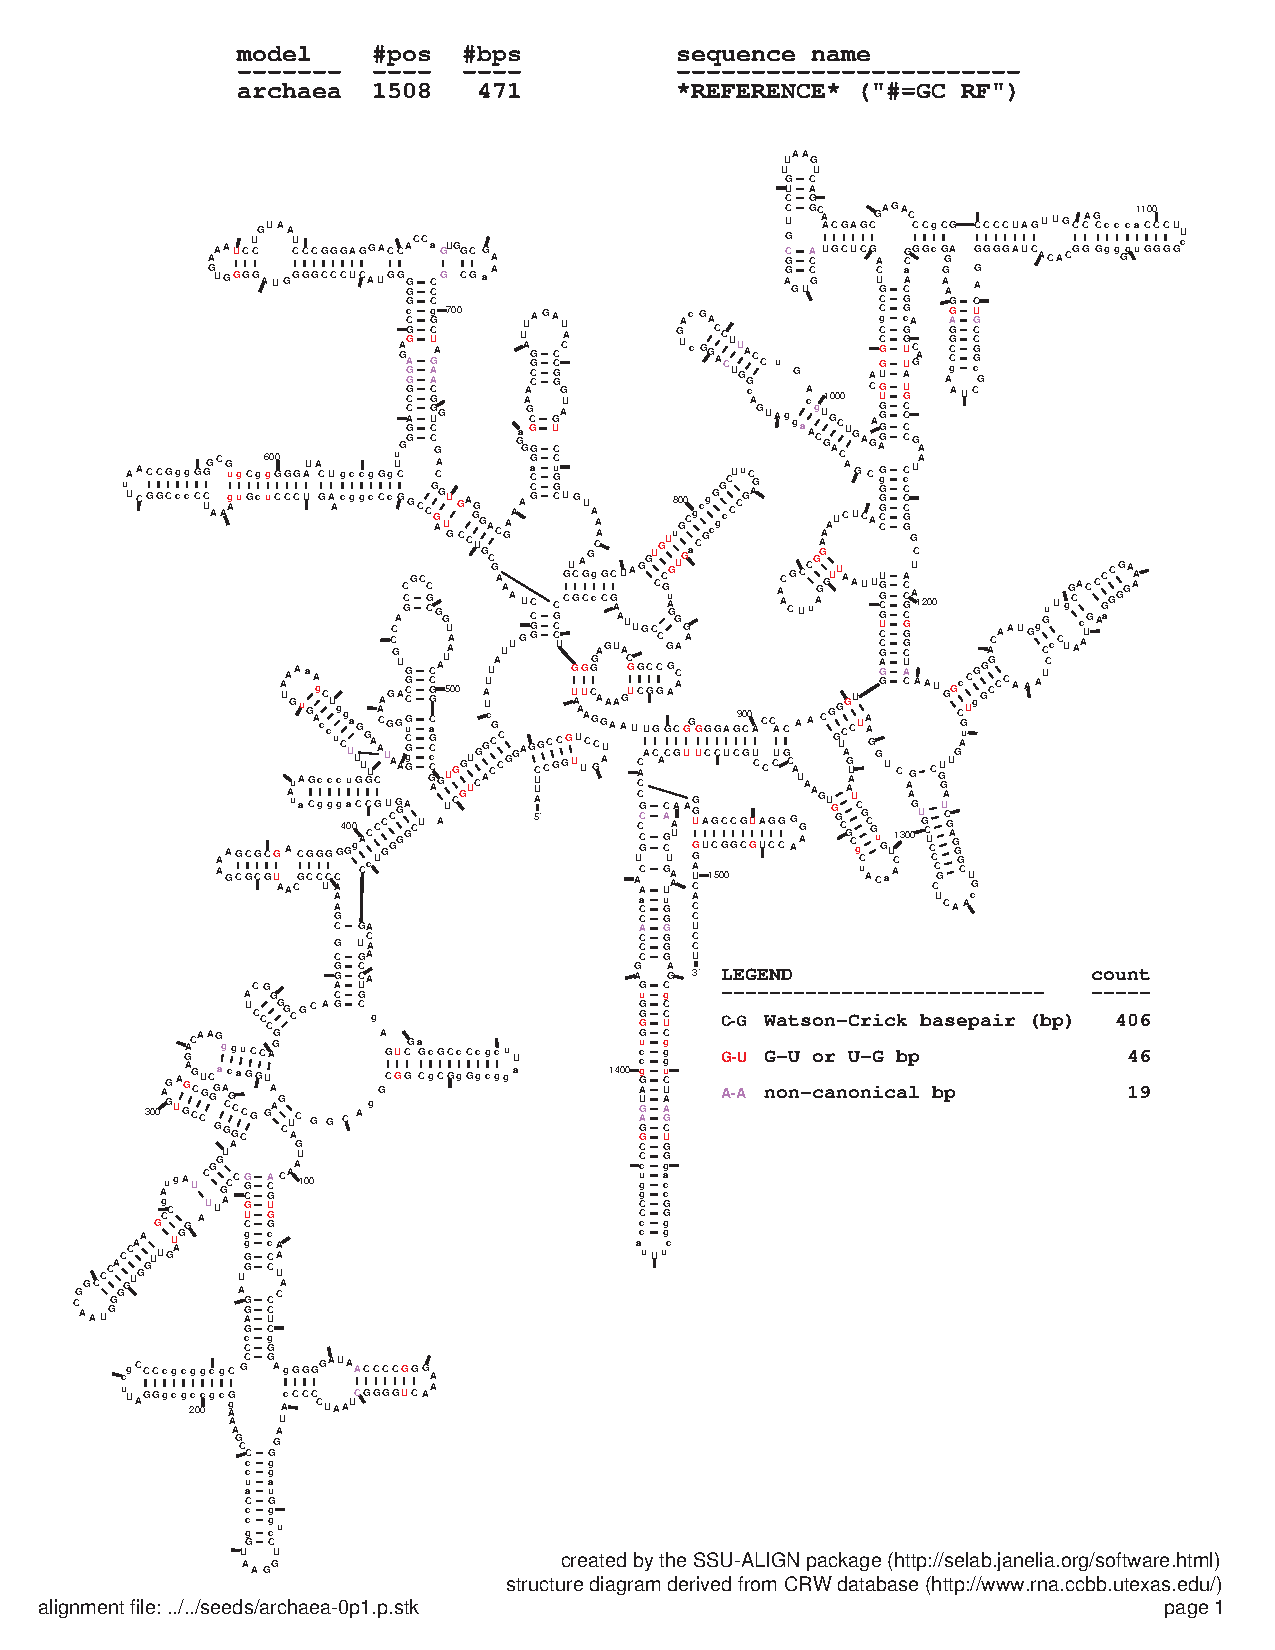
\includegraphics[width=5.7in]{Figures/archaea-0p1-rf}
\end{center}
\caption[Secondary structure diagram displaying the consensus sequence
  of the archaeal SSU model]{\textbf{Secondary structure diagram displaying the
  consensus sequence of the archaeal SSU model.} 
  This is the single sequence that the model 
  most closely represents, and is the highest scoring possible
  sequence to the model. Uppercase residues indicate highly conserved positions,
  and lowercase residues indicate less well-conserved positions.
  This diagram was generated by the {\tt
  esl-ssudraw} program included in \sft{ssu-align}.}
\label{fig:arcrf}
\end{figure}

\begin{figure}
\begin{center}
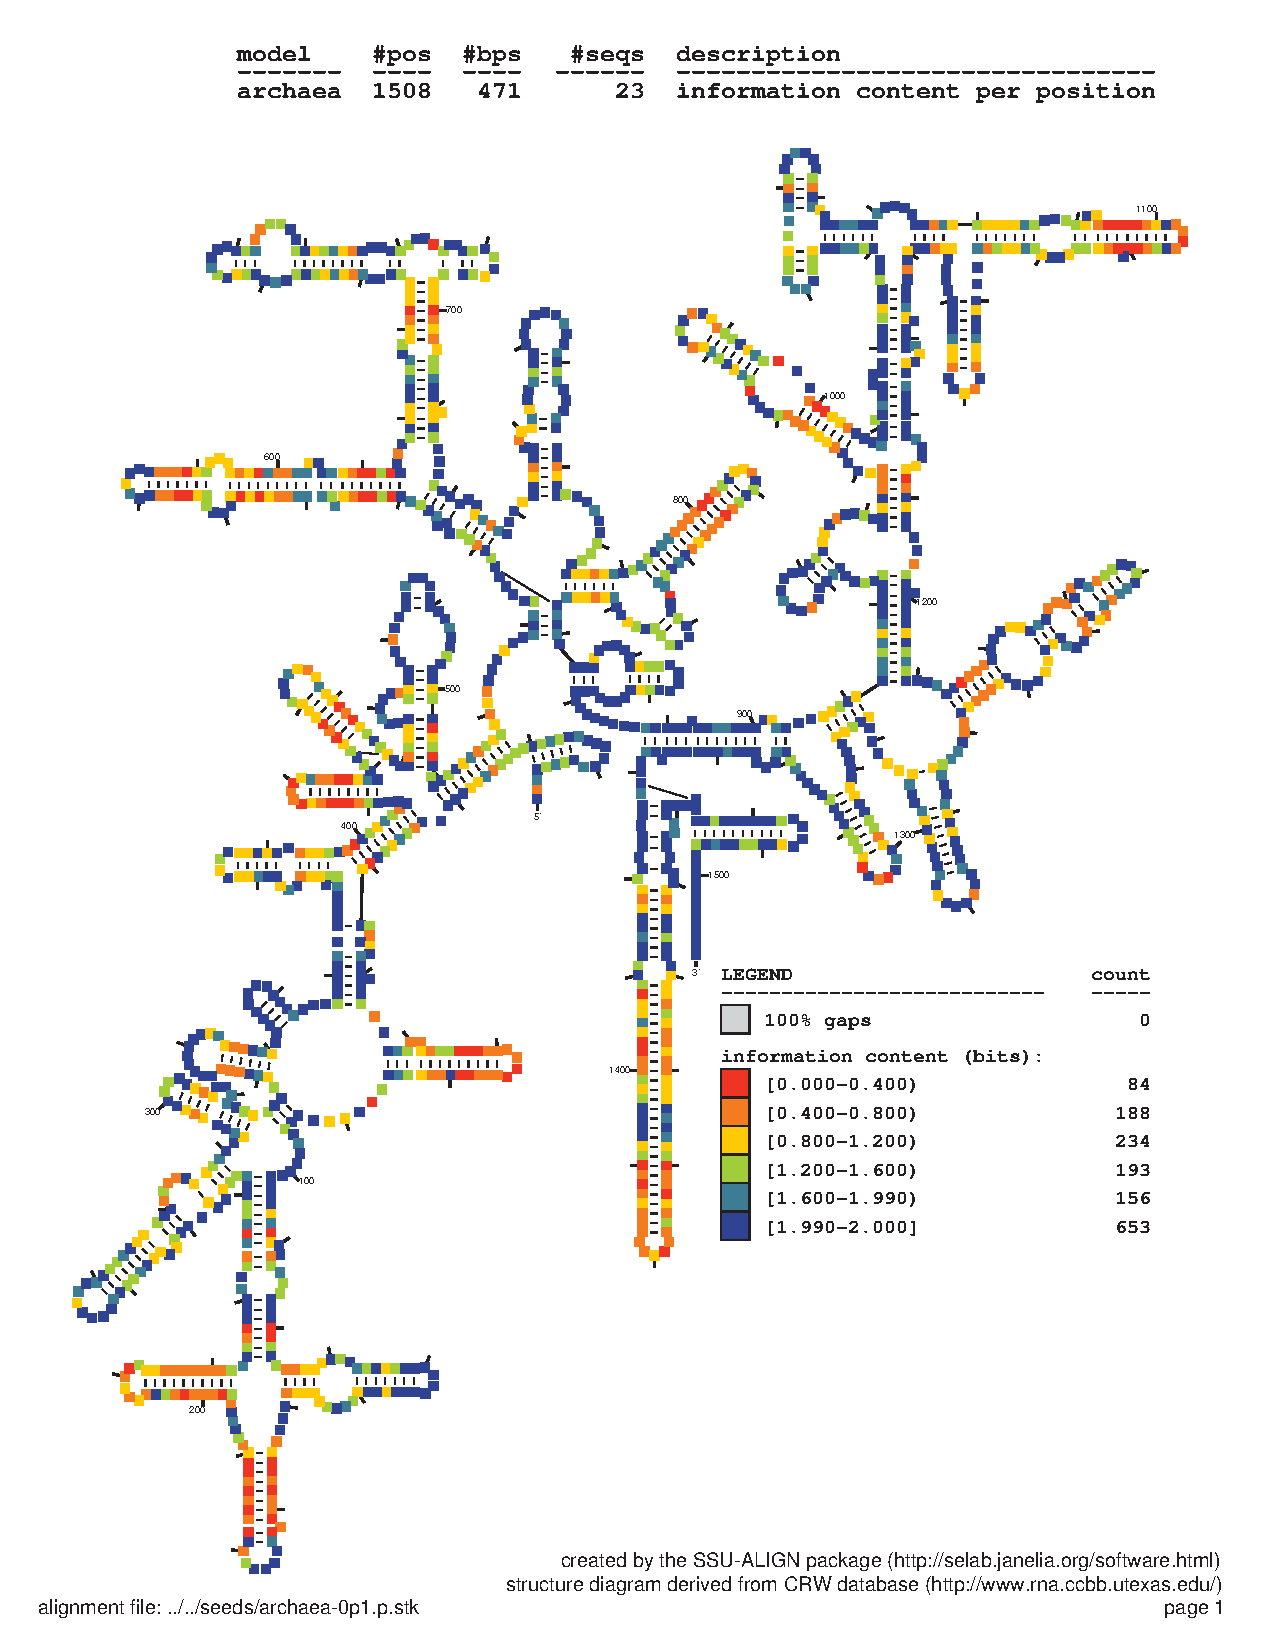
\includegraphics[width=5.7in]{Figures/archaea-0p1-info}
\end{center}
\caption[Secondary structure diagram displaying primary sequence
  information content per consensus position of the archaeal SSU seed
  alignment]{\textbf{Secondary structure diagram displaying primary
  sequence information content per consensus position of the archaeal SSU seed
  alignment.} Statistics correspond to the \sft{ssu-align} seed
  alignment derived from the \db{crw} database \cite{CannoneGutell02}
  as described in the text. This diagram was generated by the {\tt
  esl-ssudraw} program included in \sft{ssu-align}.}
\label{fig:arcinfo}
\end{figure}

\begin{figure}
\begin{center}
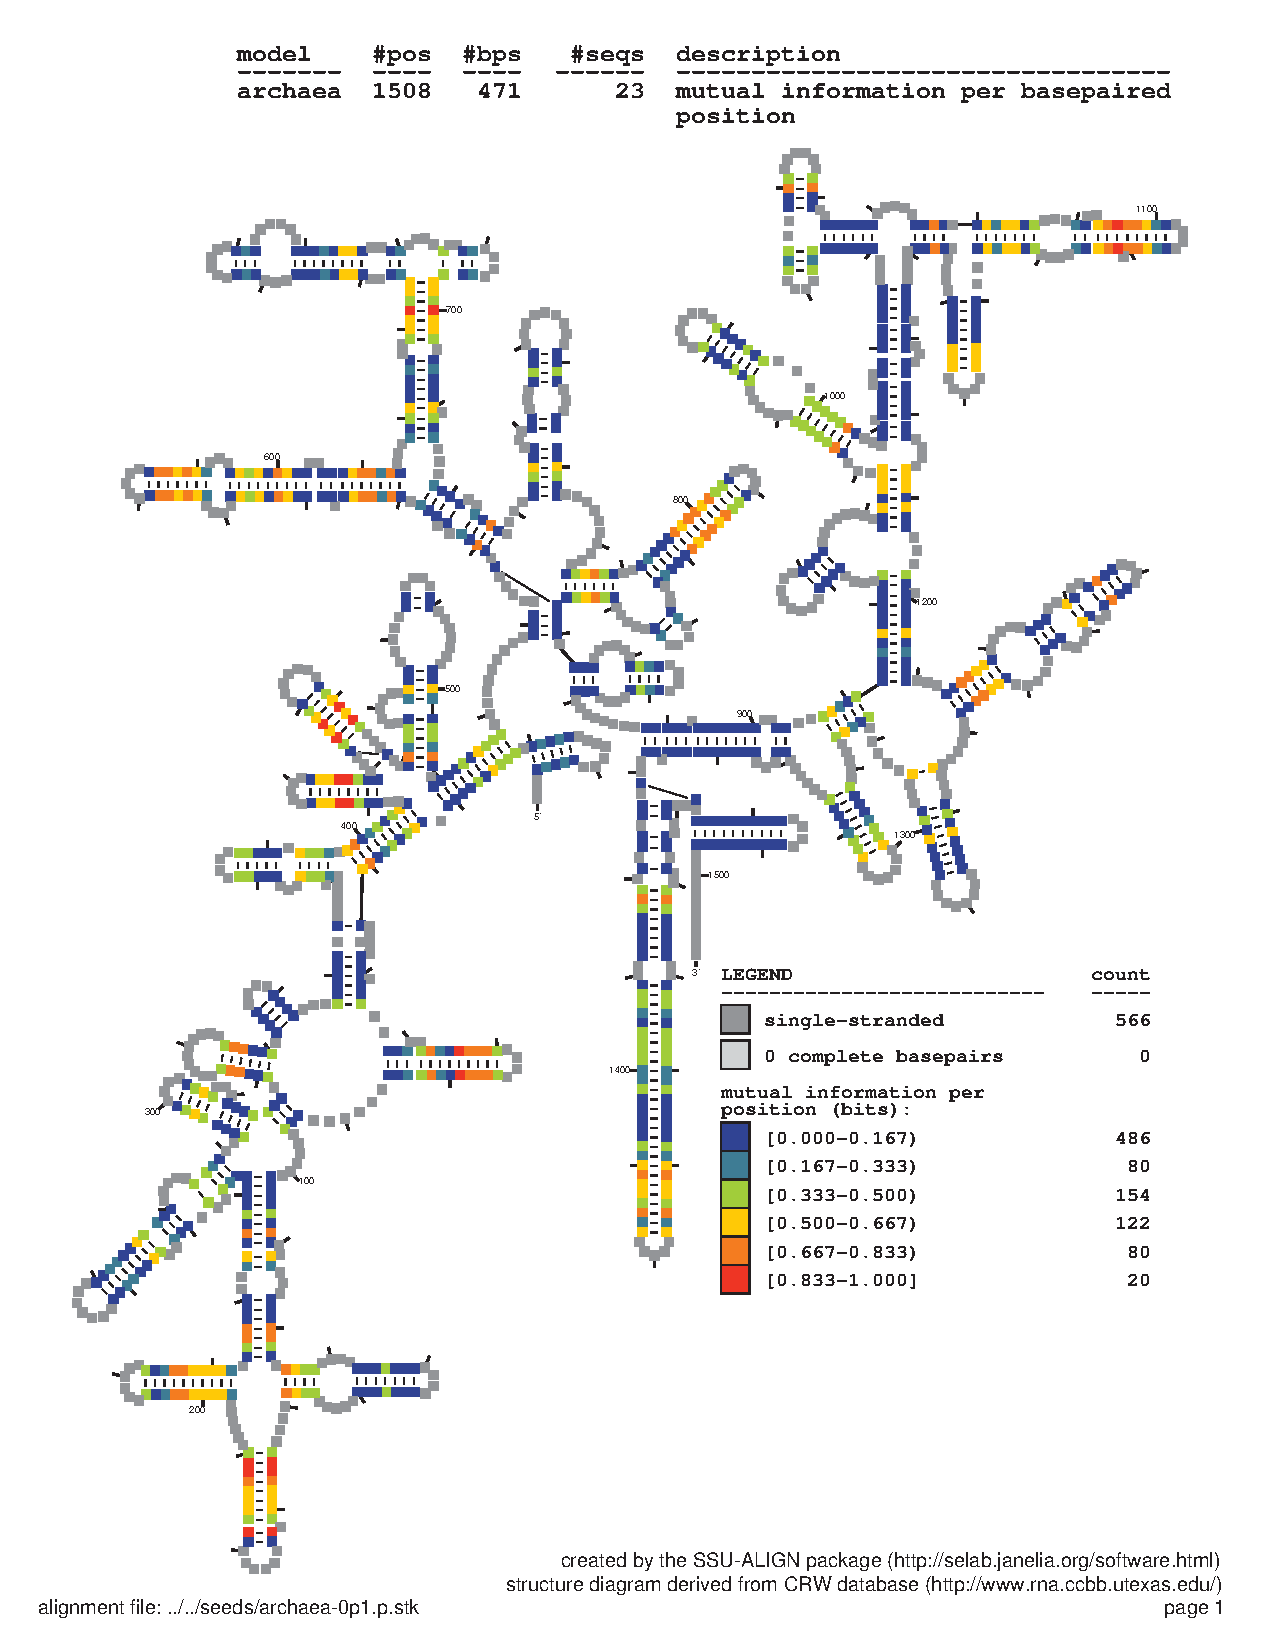
\includegraphics[width=5.7in]{Figures/archaea-0p1-mutinfo}
\end{center}
\caption[Secondary structure diagram displaying extra information 
  from conserved structure per consensus position of the archaeal SSU seed
  alignment]{\textbf{Secondary structure diagram displaying extra
  information from conserved structure per consensus position of the archaeal SSU seed
  alignment.} Statistics correspond to the \sft{ssu-align} seed
  alignment derived from the \db{crw} database \cite{CannoneGutell02}
  as described in the text. This diagram was generated by the {\tt
  esl-ssudraw} program included in \sft{ssu-align}.}
\label{fig:arcsinfo}
\end{figure}


\begin{figure}
\begin{center}
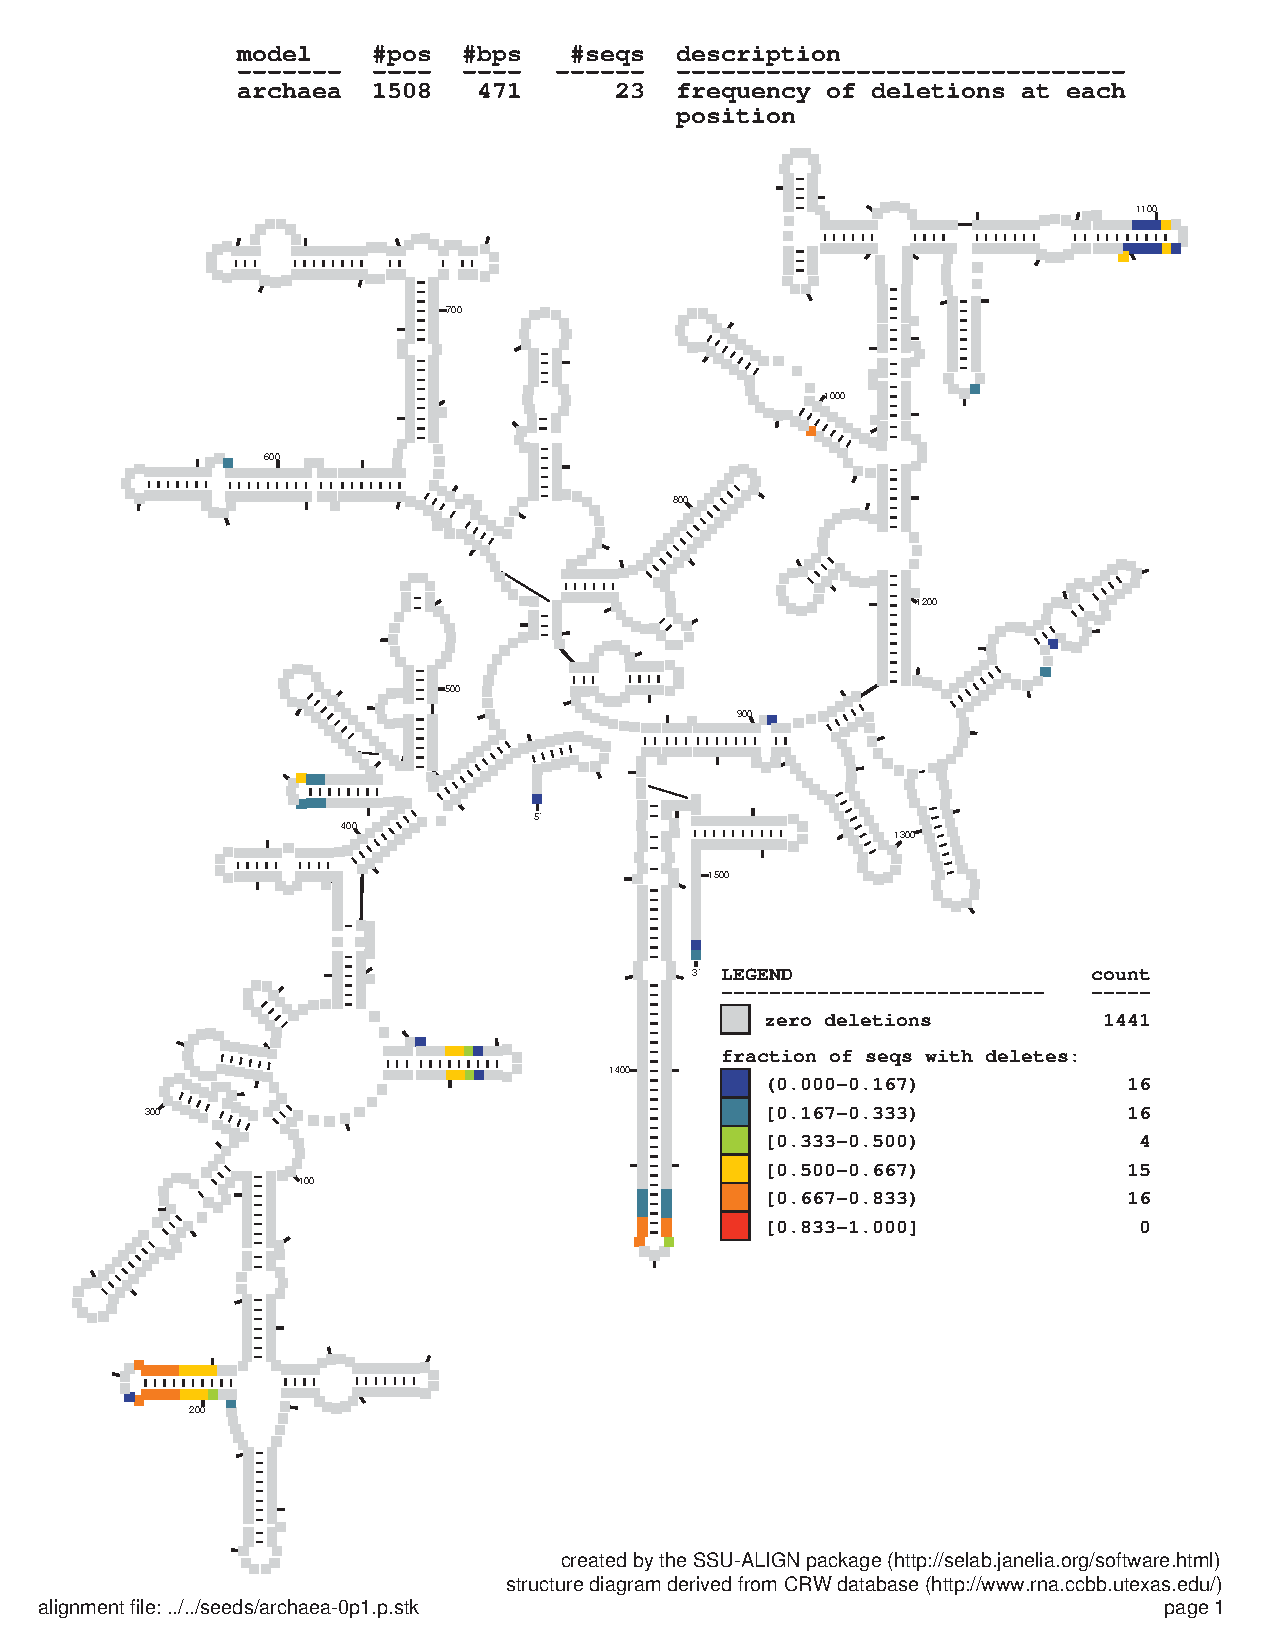
\includegraphics[width=5.7in]{Figures/archaea-0p1-dall}
\end{center}
\caption[Secondary structure diagram displaying frequency of deletions
  per consensus position of the archaeal SSU seed
  alignment]{\textbf{Secondary structure diagram displaying frequency 
  of deletions per consensus position of the archaeal SSU seed
  alignment.} Statistics correspond to the \sft{ssu-align} seed
  alignment derived from the \db{crw} database \cite{CannoneGutell02}
  as described in the text. This diagram was generated by the {\tt
  esl-ssudraw} program included in \sft{ssu-align}.}
\label{fig:arcdel}
\end{figure}


\begin{figure}
\begin{center}
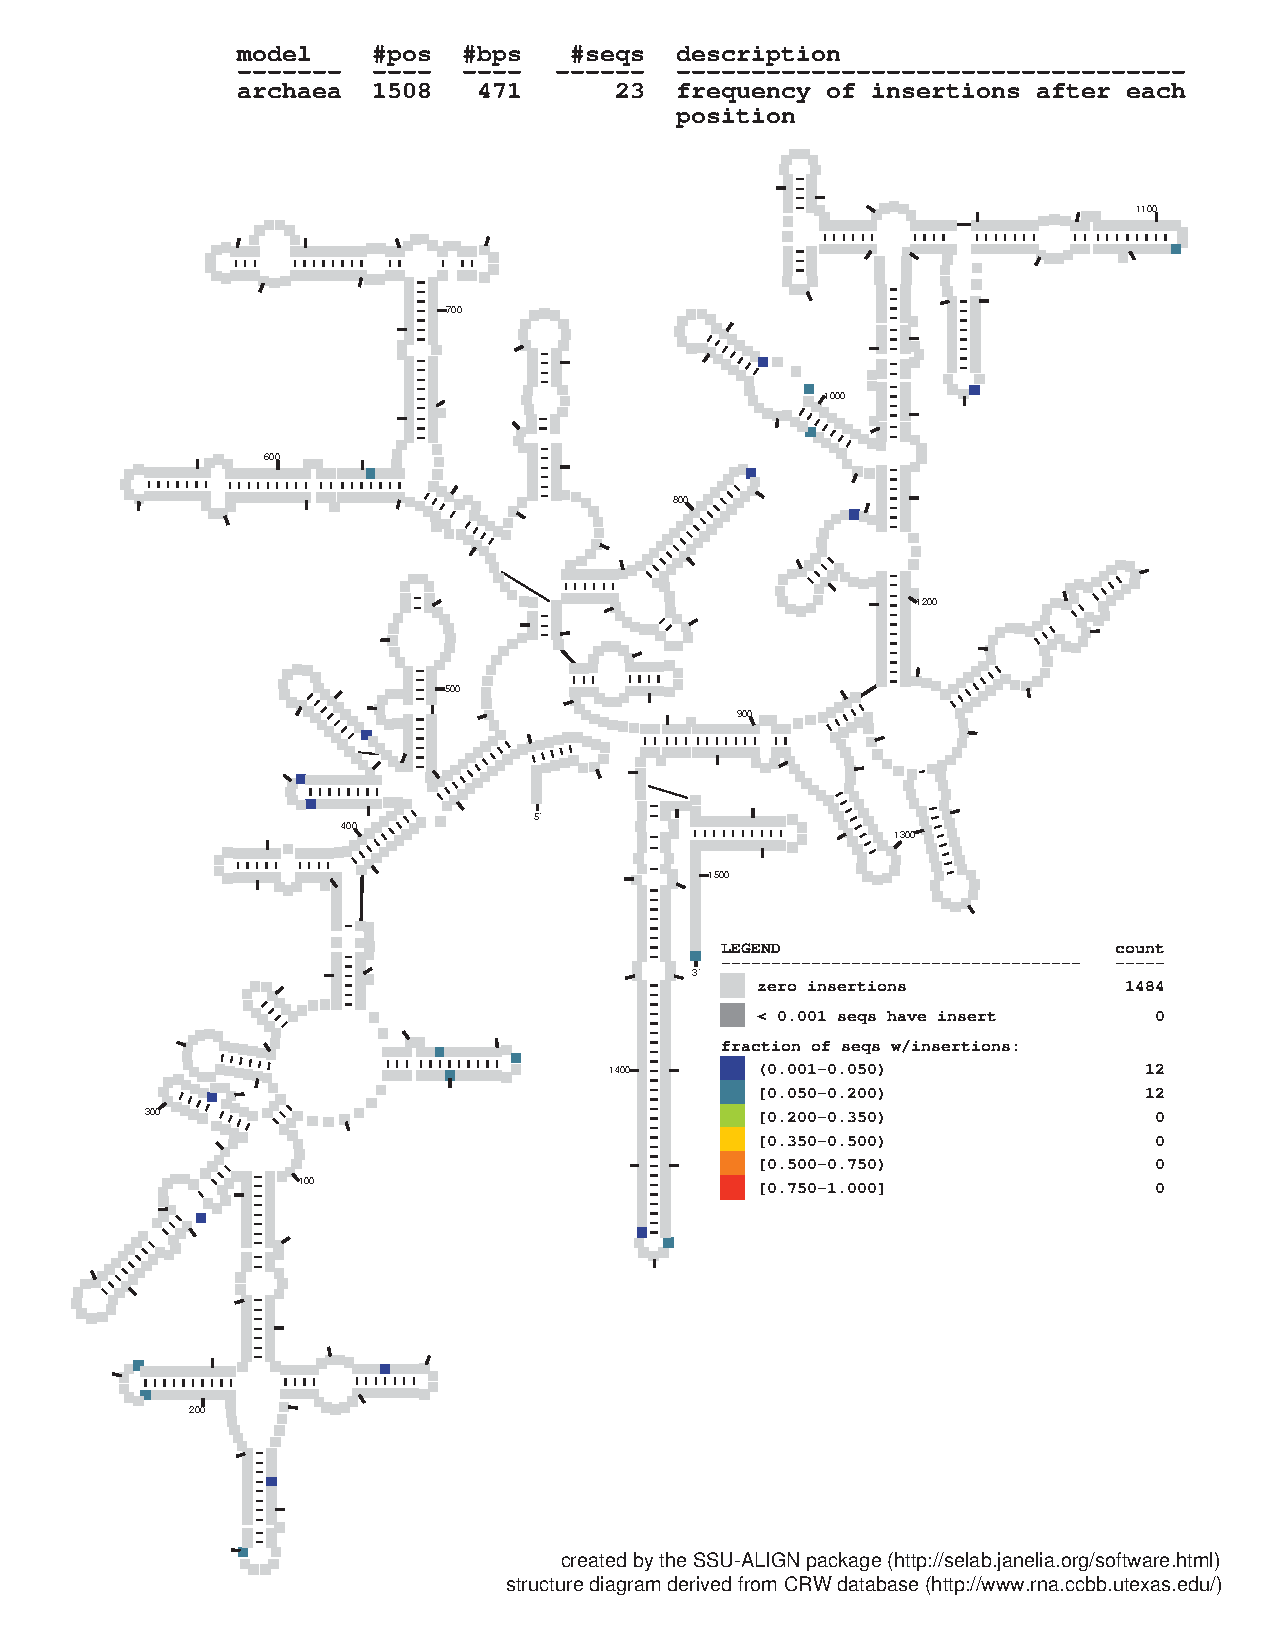
\includegraphics[width=5.7in]{Figures/archaea-0p1-ifreq}
\end{center}
\caption[Secondary structure diagram displaying frequency of insertions
  after each consensus position in the archaeal SSU seed
  alignment]{\textbf{Secondary structure diagram displaying frequency
  of insertions after each consensus position in the archaeal SSU seed
  alignment.} Statistics correspond to the \sft{ssu-align} seed
  alignment derived from the \db{crw} database \cite{CannoneGutell02}
  as described in the text. This diagram was generated by the {\tt
  esl-ssudraw} program included in \sft{ssu-align}.}
\label{fig:arcins}
\end{figure}


%%%%%%%%%%%%%%%%%%%%%%%%%%%%%%%%%%%%%%%%%%%%%%%%%%%%%%%%%%%%%%%%
%bacteria
%%%%%%%%%%%%%%%%%%%%%%%%%%%%%%%%%%%%%%%%%%%%%%%%%%%%%%%%%%%%%%%%
\begin{figure}
\begin{center}
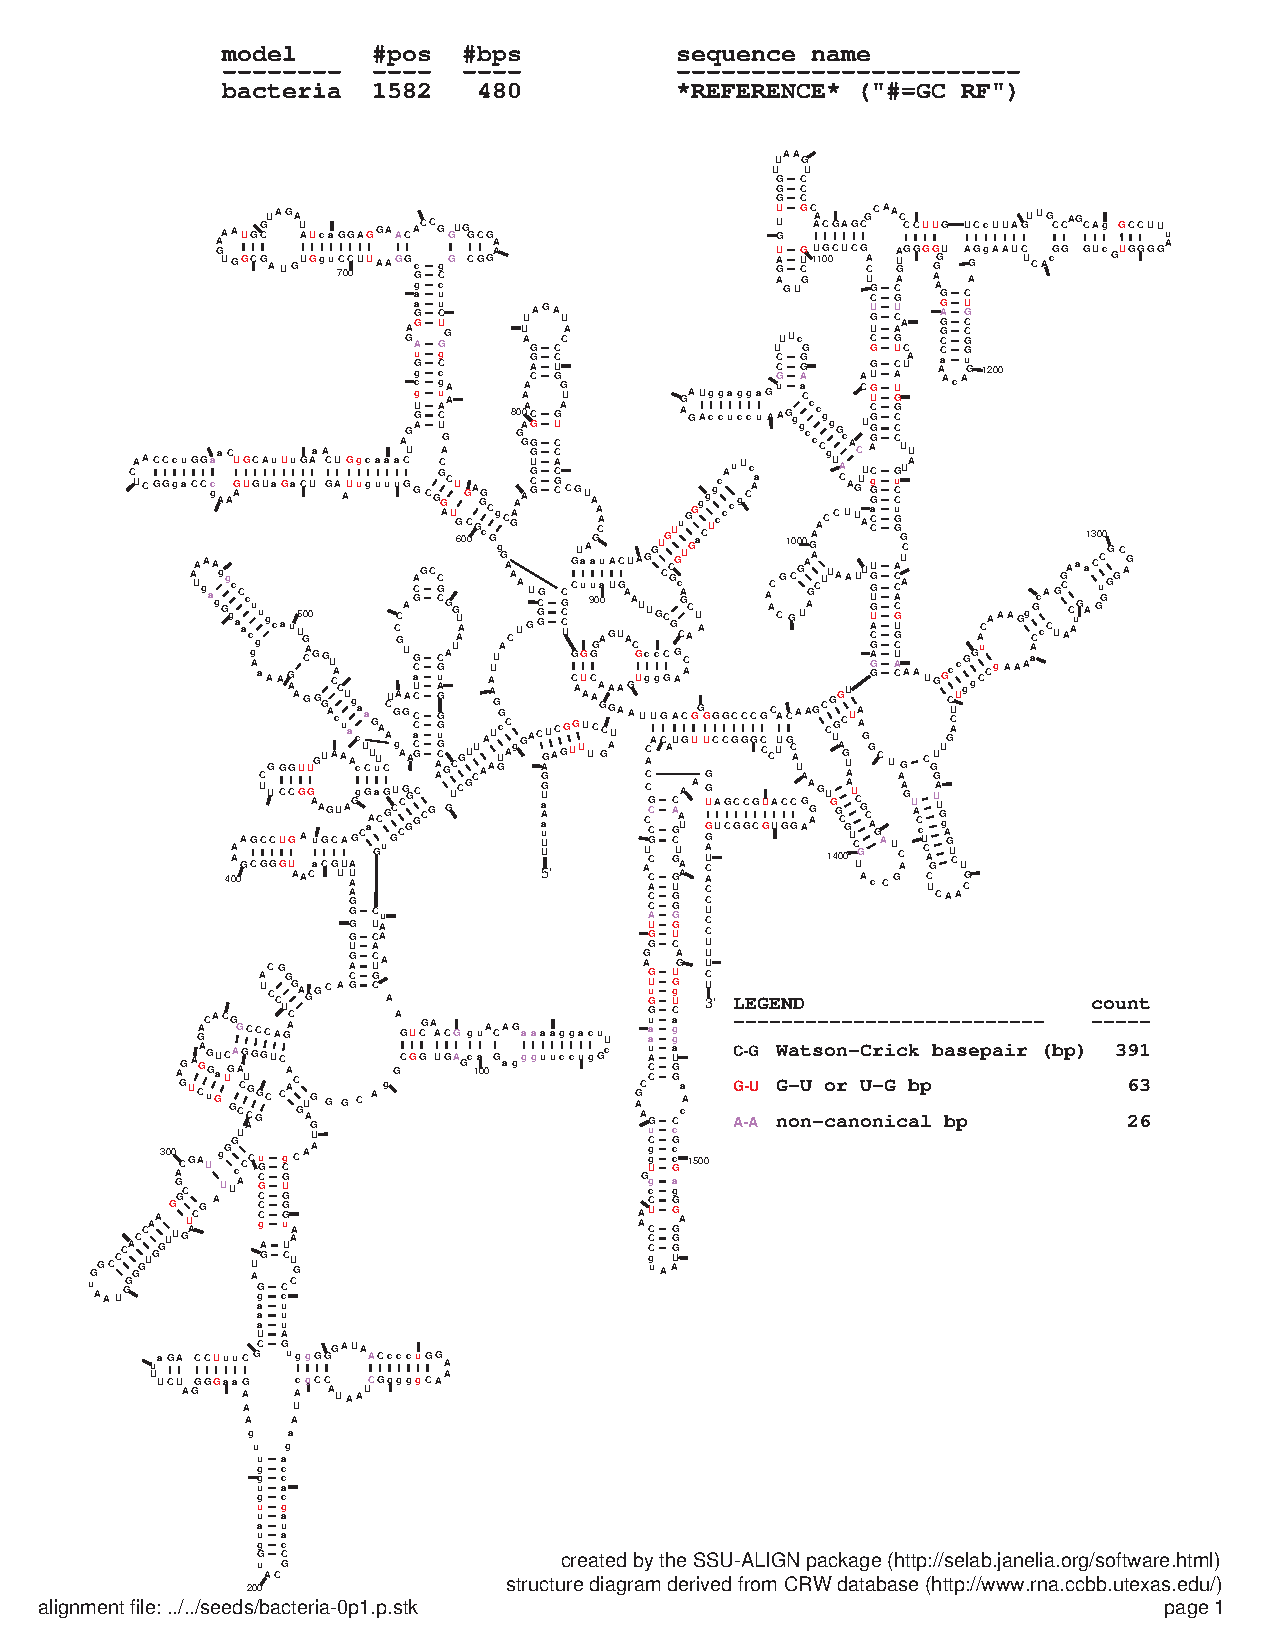
\includegraphics[width=5.7in]{Figures/bacteria-0p1-rf}
\end{center}
\caption[Secondary structure diagram displaying the consensus sequence
  of the bacterial SSU model]{\textbf{Secondary structure diagram displaying the
  consensus sequence of the bacterial SSU model.} 
  This is the single sequence that the model 
  most closely represents, and is the highest scoring possible
  sequence to the model. Uppercase residues indicate highly conserved positions,
  and lowercase residues indicate less well-conserved positions.
  This diagram was generated by the {\tt
  esl-ssudraw} program included in \sft{ssu-align}.}
\label{fig:bacrf}
\end{figure}

\begin{figure}
\begin{center}
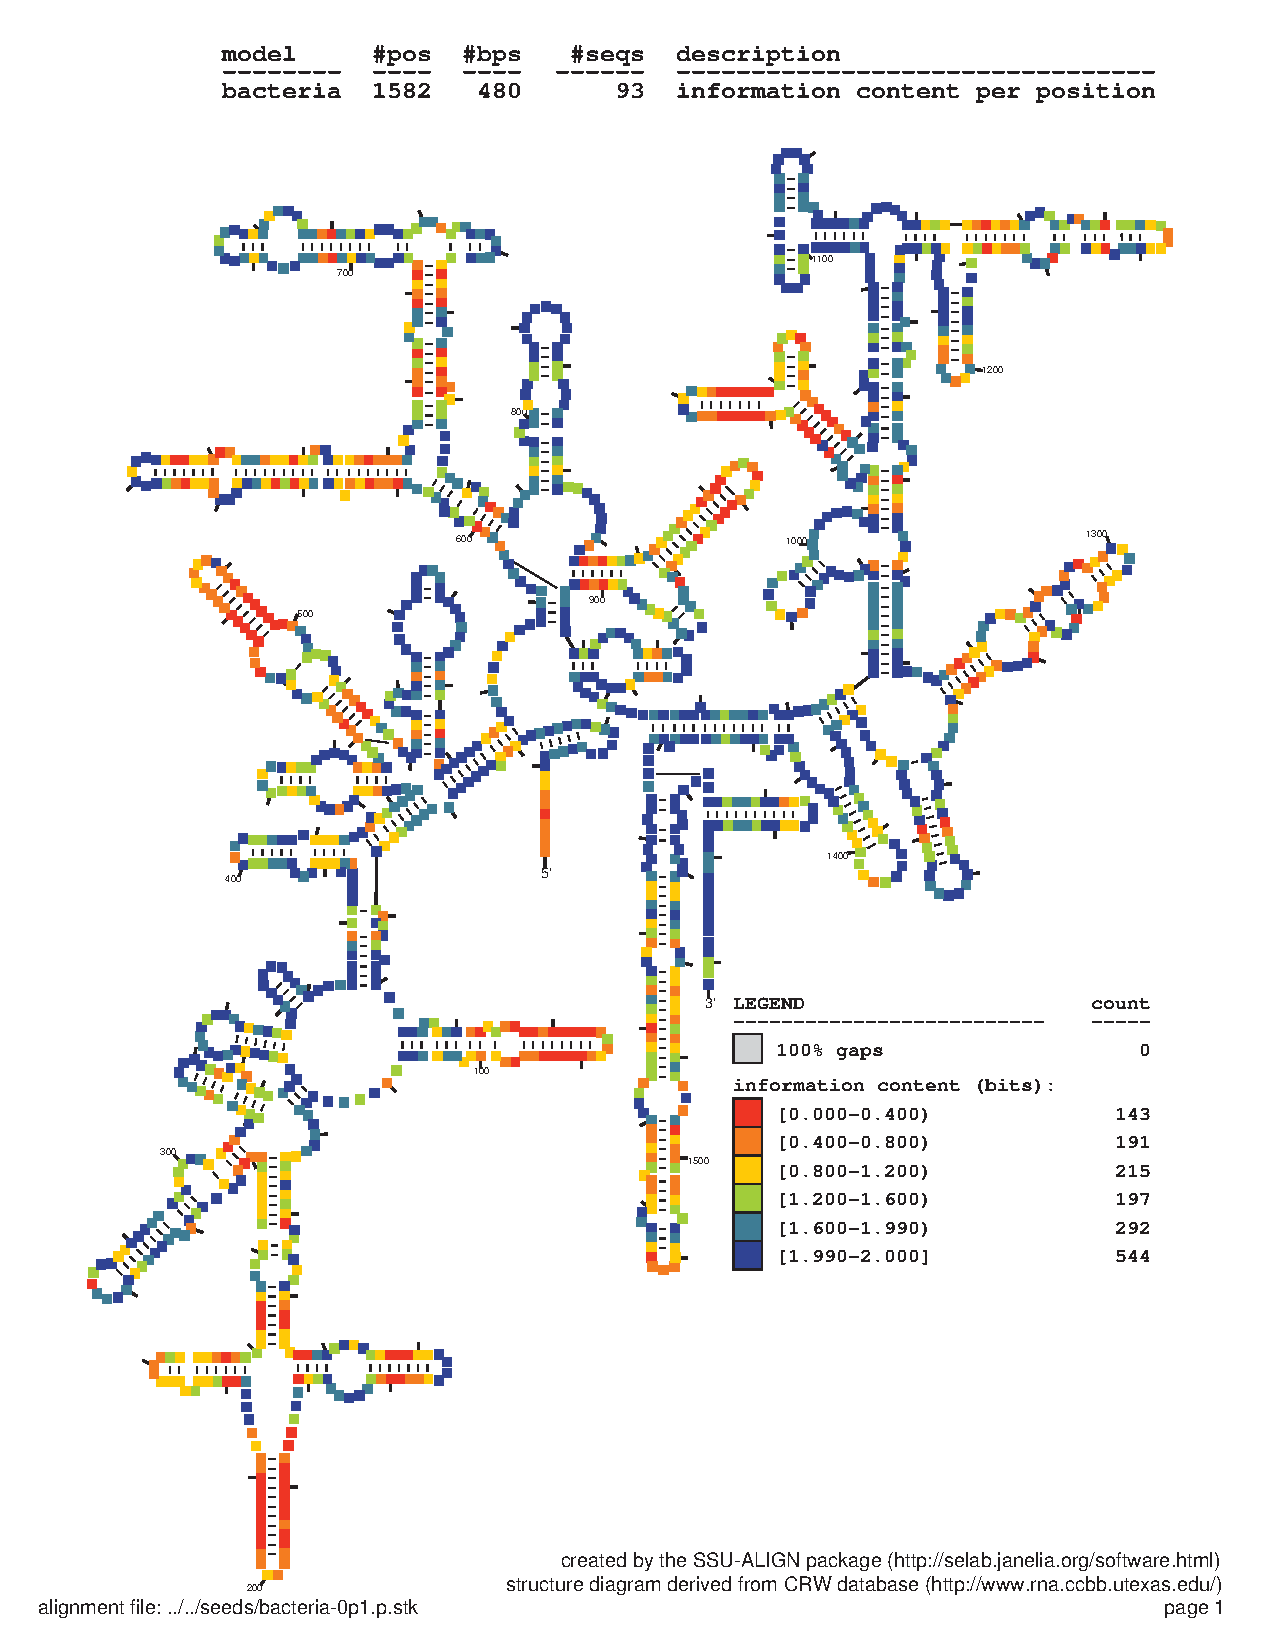
\includegraphics[width=5.7in]{Figures/bacteria-0p1-info}
\end{center}
\caption[Secondary structure diagram displaying primary sequence
  information content per consensus position of the bacterial SSU seed
  alignment]{\textbf{Secondary structure diagram displaying primary
  sequence information content per consensus position of the bacterial SSU seed
  alignment.} Statistics correspond to the \sft{ssu-align} seed
  alignment derived from the \db{crw} database \cite{CannoneGutell02}
  as described in the text. This diagram was generated by the {\tt
  esl-ssudraw} program included in \sft{ssu-align}.}
\label{fig:bacinfo}
\end{figure}


\begin{figure}
\begin{center}
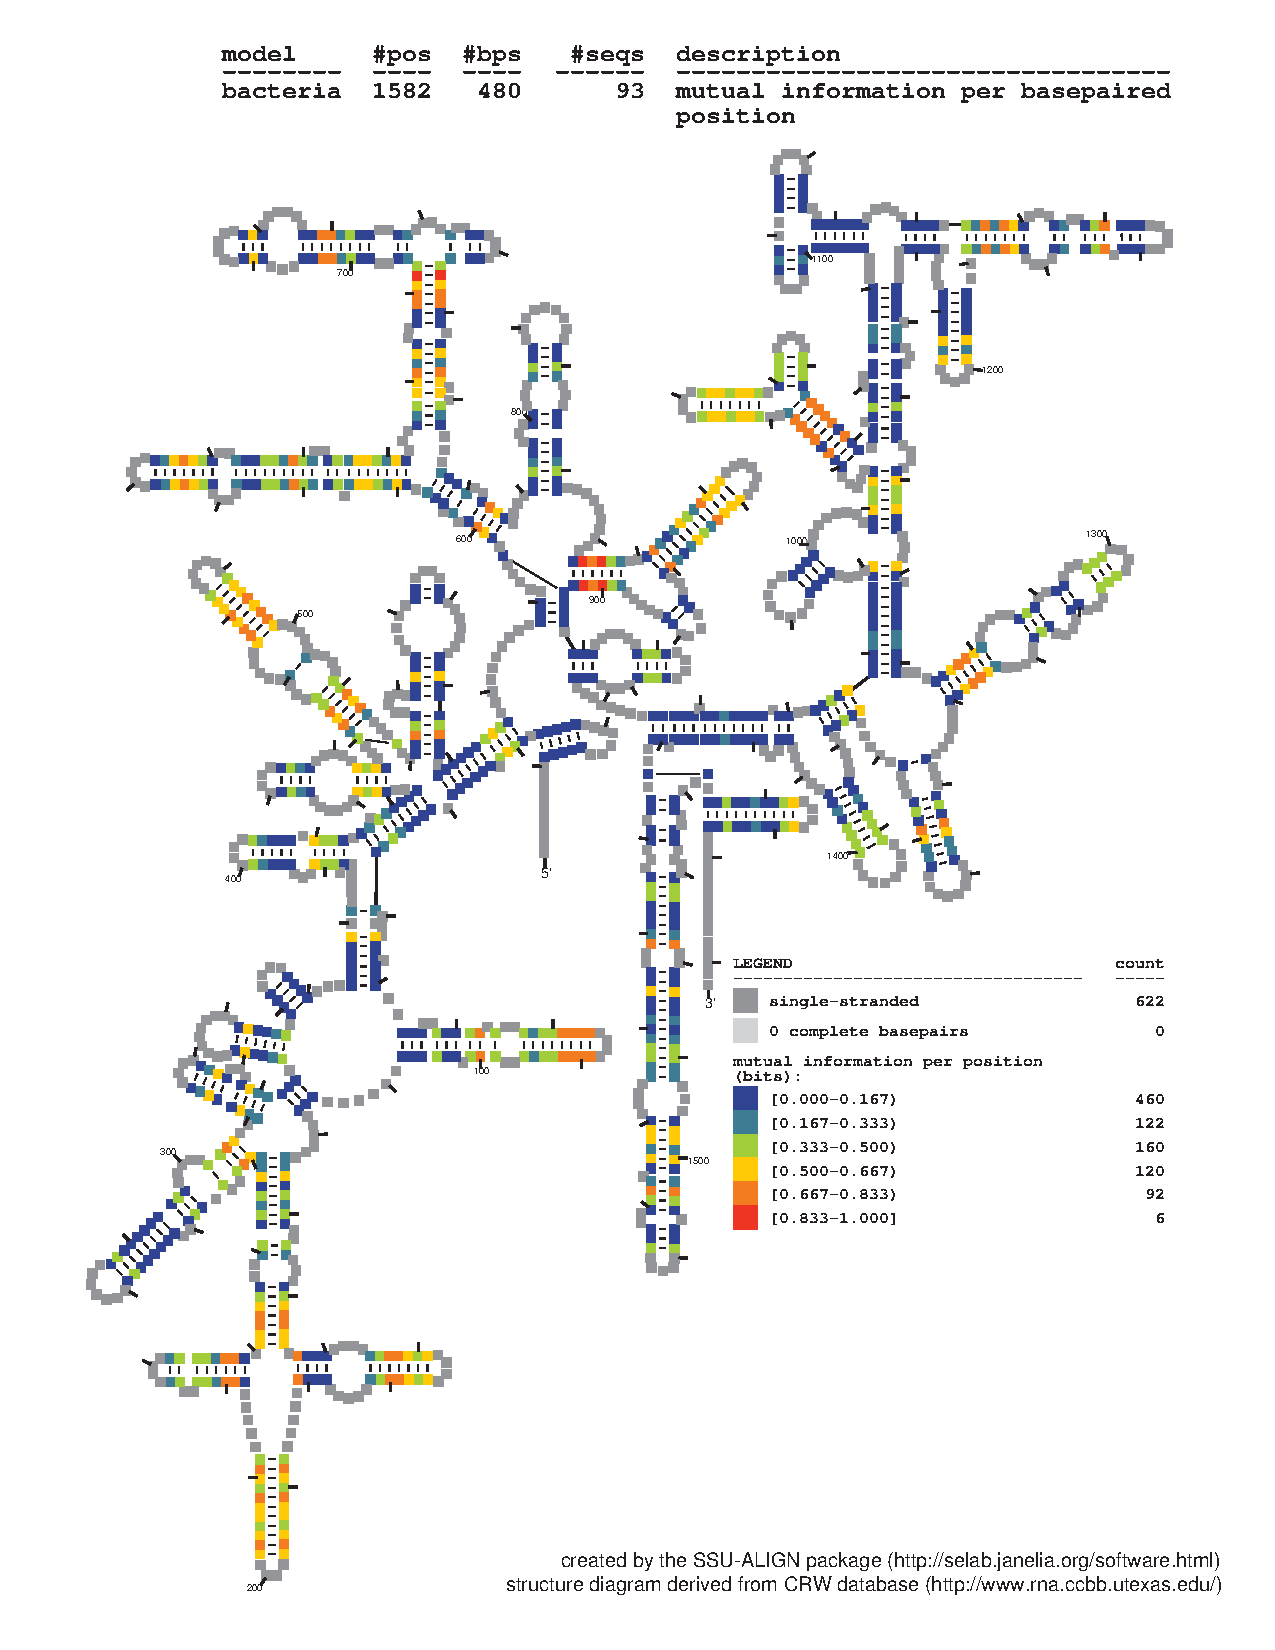
\includegraphics[width=5.7in]{Figures/bacteria-0p1-mutinfo}
\end{center}
\caption[Secondary structure diagram displaying extra information 
  from conserved structure per consensus position of the bacterial SSU seed
  alignment]{\textbf{Secondary structure diagram displaying extra
  information from conserved structure per consensus position of the bacterial SSU seed
  alignment.} Statistics correspond to the \sft{ssu-align} seed
  alignment derived from the \db{crw} database \cite{CannoneGutell02}
  as described in the text. This diagram was generated by the {\tt
  esl-ssudraw} program included in \sft{ssu-align}.}
\label{fig:bacsinfo}
\end{figure}


\begin{figure}
\begin{center}
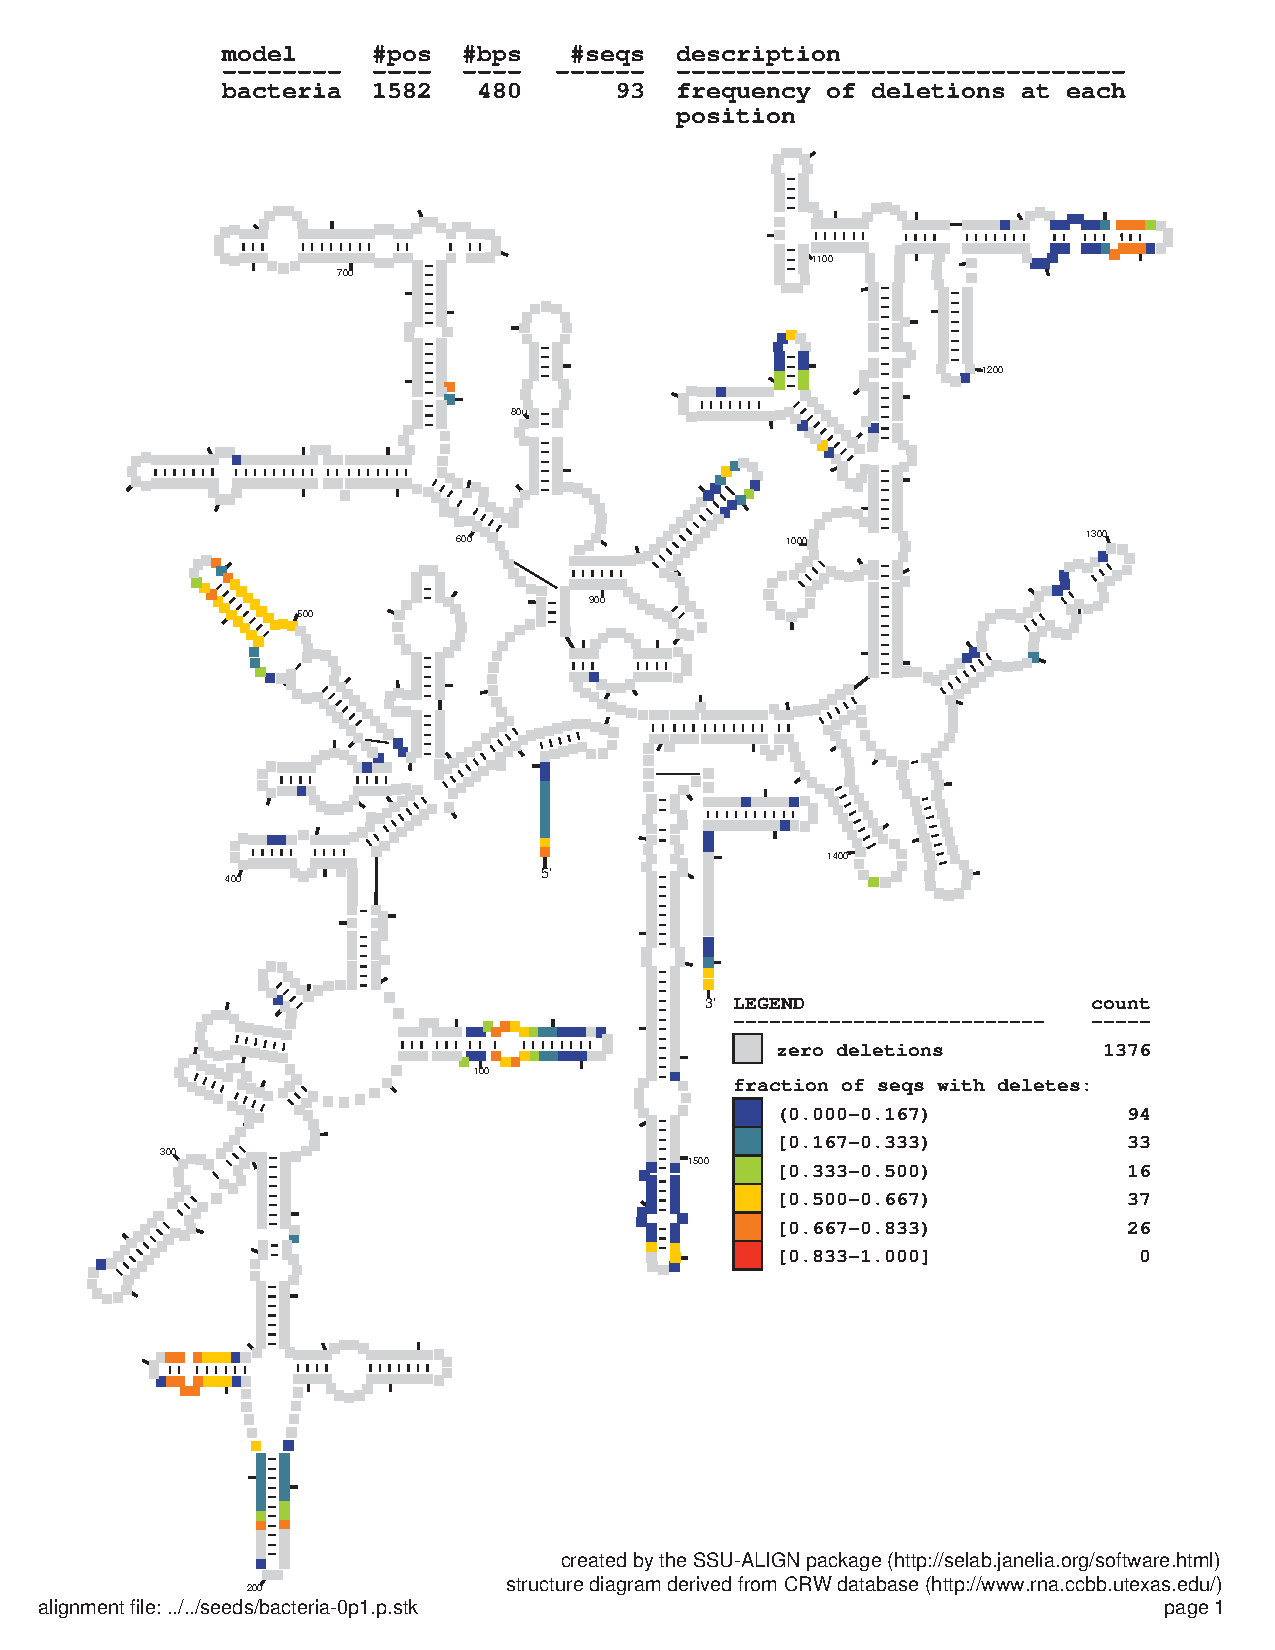
\includegraphics[width=5.7in]{Figures/bacteria-0p1-dall}
\end{center}
\caption[Secondary structure diagram displaying frequency of deletions
  per consensus position of the bacterial SSU seed
  alignment]{\textbf{Secondary structure diagram displaying frequency 
  of deletions per consensus position of the bacterial SSU seed
  alignment.} Statistics correspond to the \sft{ssu-align} seed
  alignment derived from the \db{crw} database \cite{CannoneGutell02}
  as described in the text. This diagram was generated by the {\tt
  esl-ssudraw} program included in \sft{ssu-align}.}
\label{fig:bacdel}
\end{figure}


\begin{figure}
\begin{center}
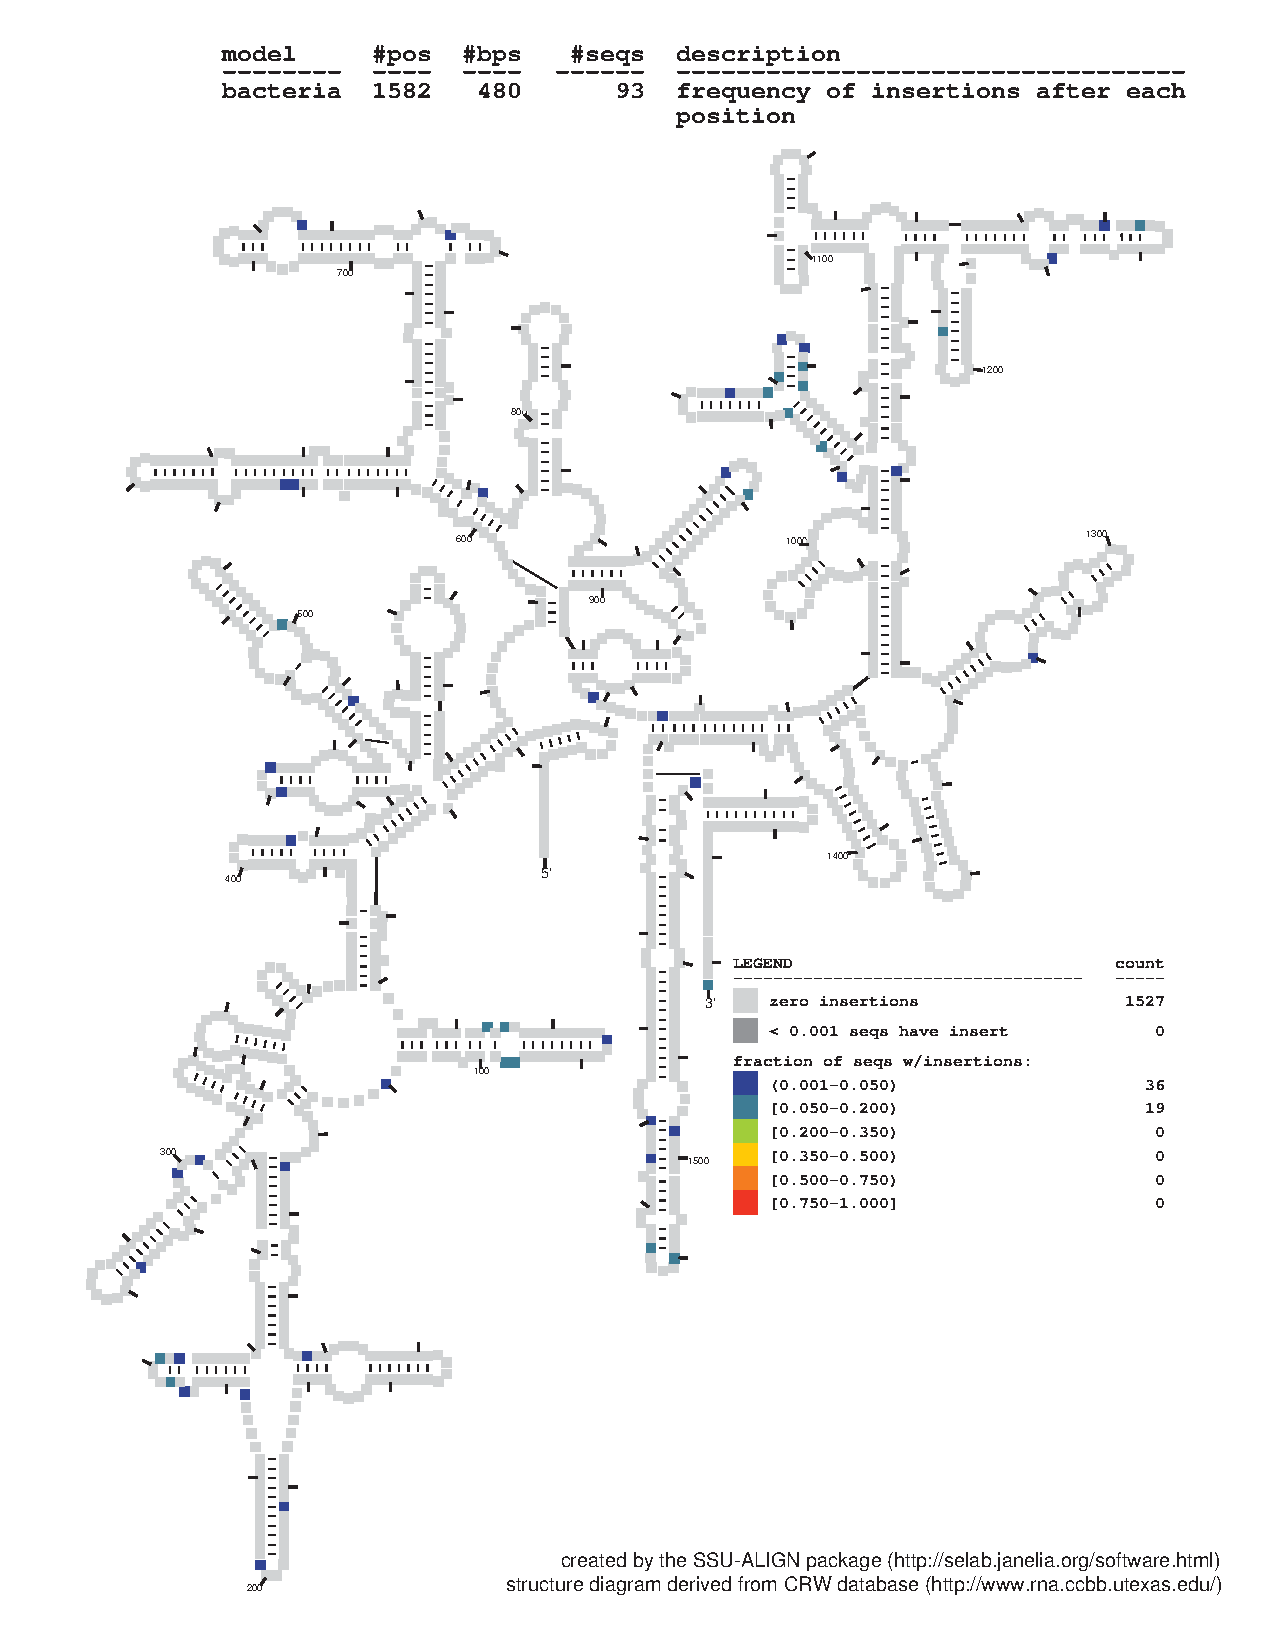
\includegraphics[width=5.7in]{Figures/bacteria-0p1-ifreq}
\end{center}
\caption[Secondary structure diagram displaying frequency of insertions
  after each consensus position in the bacterial SSU seed
  alignment]{\textbf{Secondary structure diagram displaying frequency
  of insertions after each consensus position in the bacterial SSU seed
  alignment.} Statistics correspond to the \sft{ssu-align} seed
  alignment derived from the \db{crw} database \cite{CannoneGutell02}
  as described in the text. This diagram was generated by the {\tt
  esl-ssudraw} program included in \sft{ssu-align}.}
\label{fig:bacins}
\end{figure}




%%%%%%%%%%%%%%%%%%%%%%%%%%%%%%%%%%%%%%%%%%%%%%%%%%%%%%%%%%%%%%%%
%eukarya
%%%%%%%%%%%%%%%%%%%%%%%%%%%%%%%%%%%%%%%%%%%%%%%%%%%%%%%%%%%%%%%%
\begin{figure}
\begin{center}
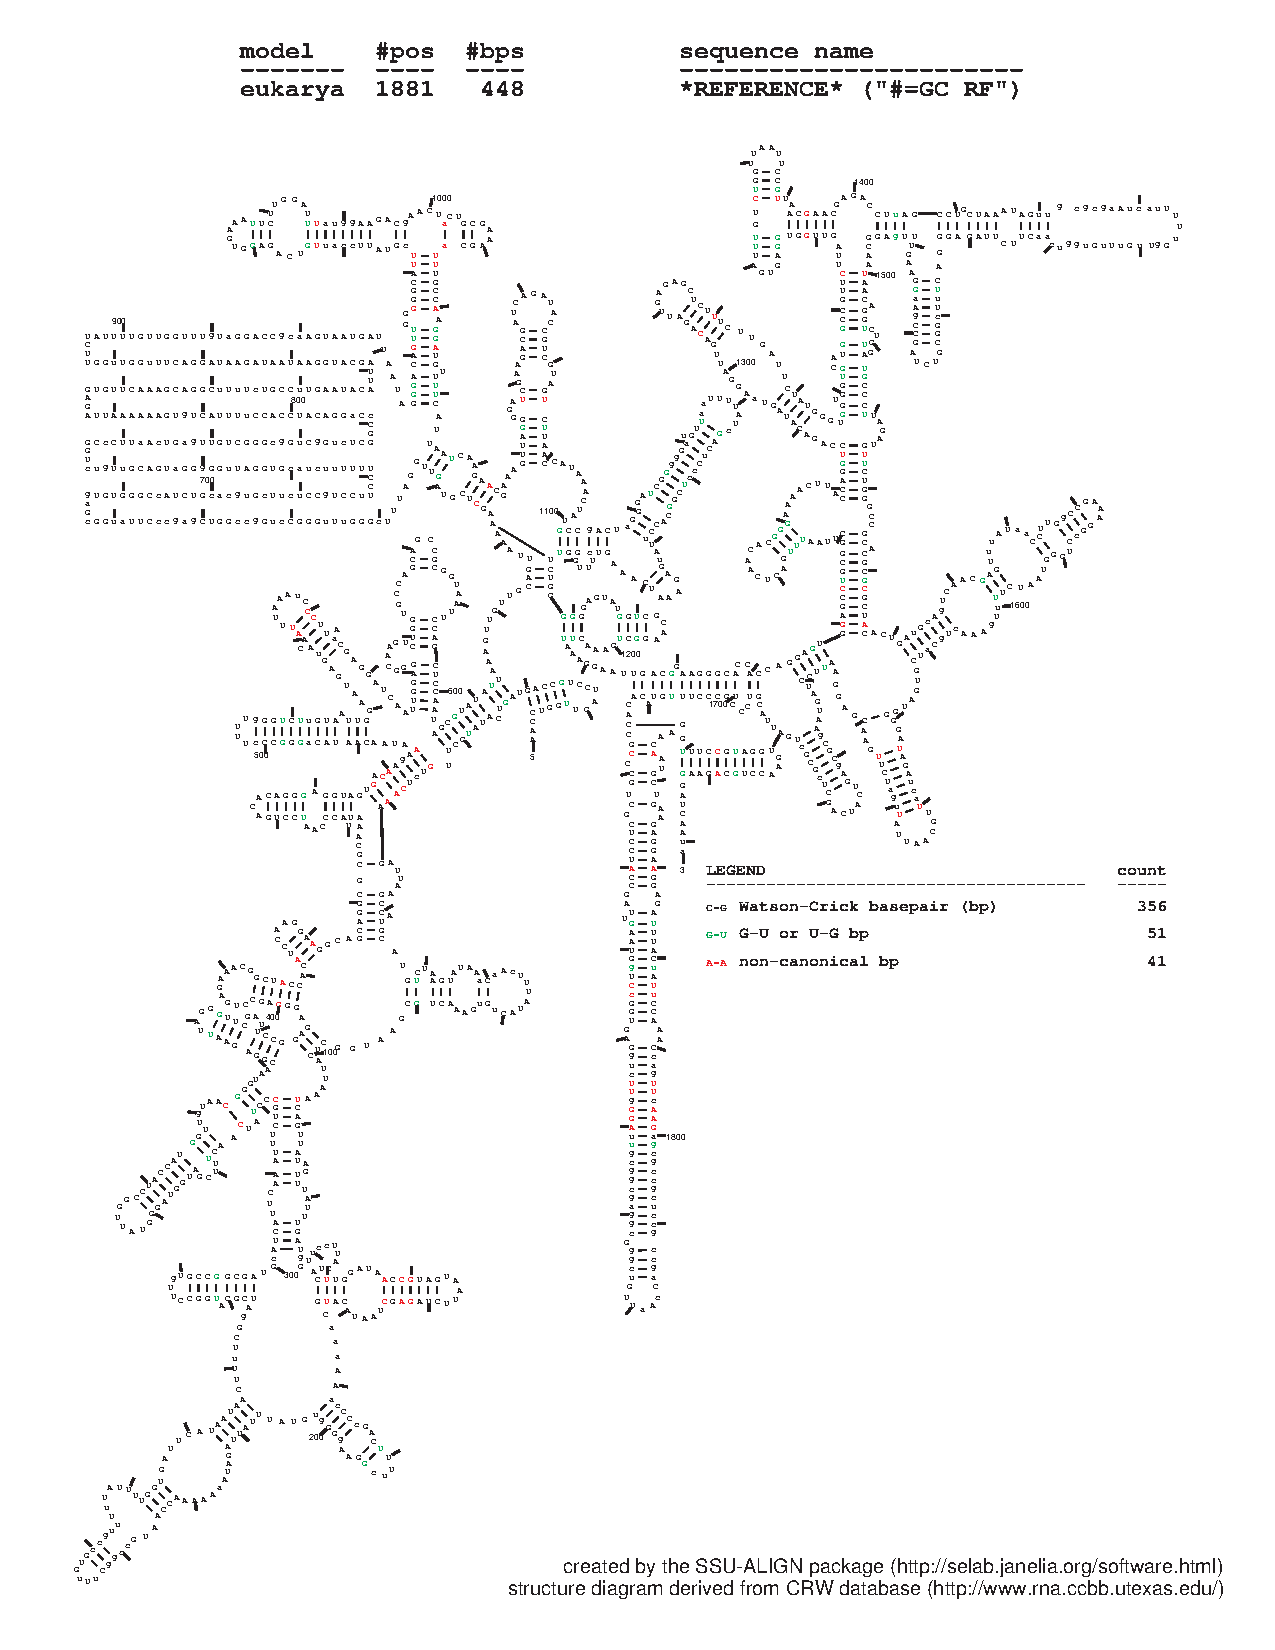
\includegraphics[width=5.7in]{Figures/eukarya-0p1-rf}
\end{center}
\caption[Secondary structure diagram displaying the consensus sequence
  of the eukaryotic SSU model]{\textbf{Secondary structure diagram displaying the
  consensus sequence of the eukaryotic SSU model.} 
  This is the single sequence that the model 
  most closely represents, and is the highest scoring possible
  sequence to the model. Uppercase residues indicate highly conserved positions,
  and lowercase residues indicate less well-conserved positions.
  This diagram was generated by the {\tt
  esl-ssudraw} program included in \sft{ssu-align}.}
\label{fig:eukrf}
\end{figure}

\begin{figure}
\begin{center}
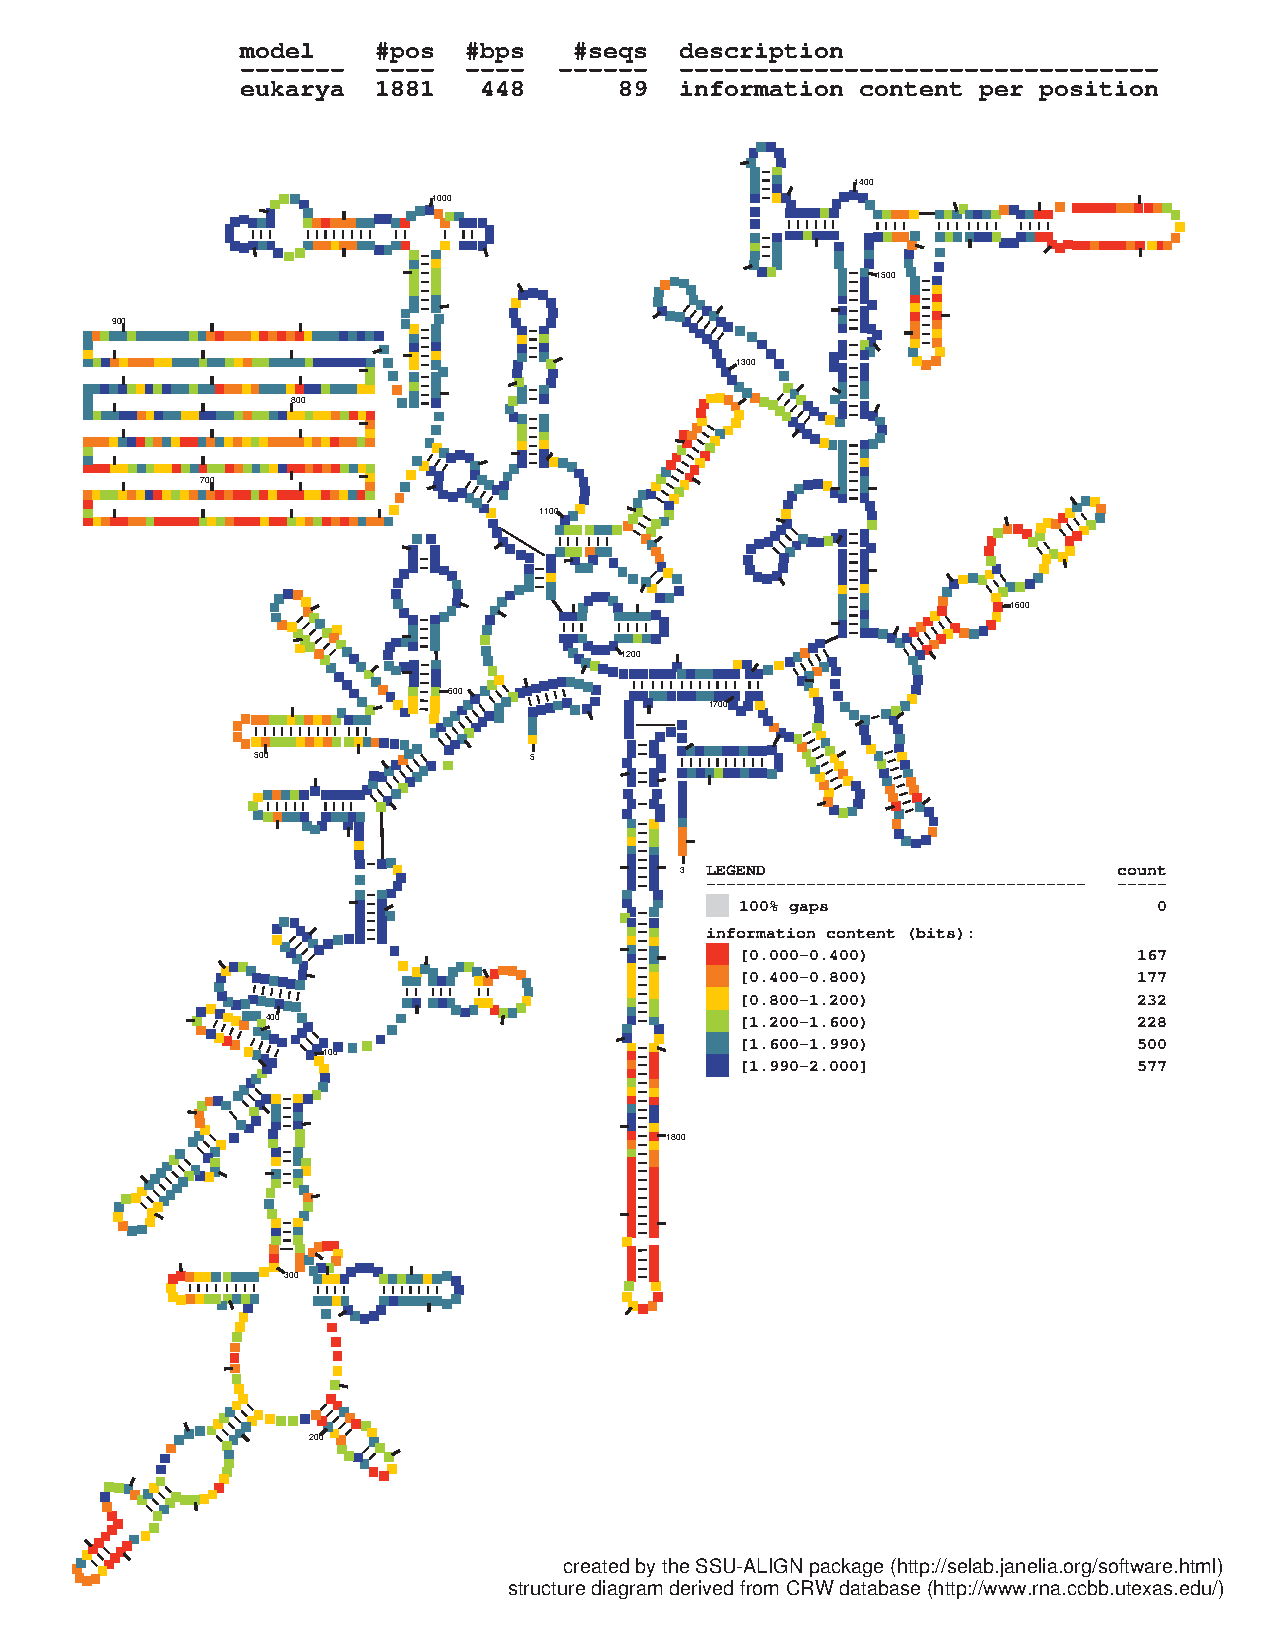
\includegraphics[width=5.7in]{Figures/eukarya-0p1-info}
\end{center}
\caption[Secondary structure diagram displaying primary sequence
  information content per consensus position of the eukaryotic SSU seed
  alignment]{\textbf{Secondary structure diagram displaying primary
  sequence information content per consensus position of the eukaryotic SSU seed
  alignment.} Statistics correspond to the \sft{ssu-align} seed
  alignment derived from the \db{crw} database \cite{CannoneGutell02}
  as described in the text. This diagram was generated by the {\tt
  esl-ssudraw} program included in \sft{ssu-align}.}
\label{fig:eukinfo}
\end{figure}


\begin{figure}
\begin{center}
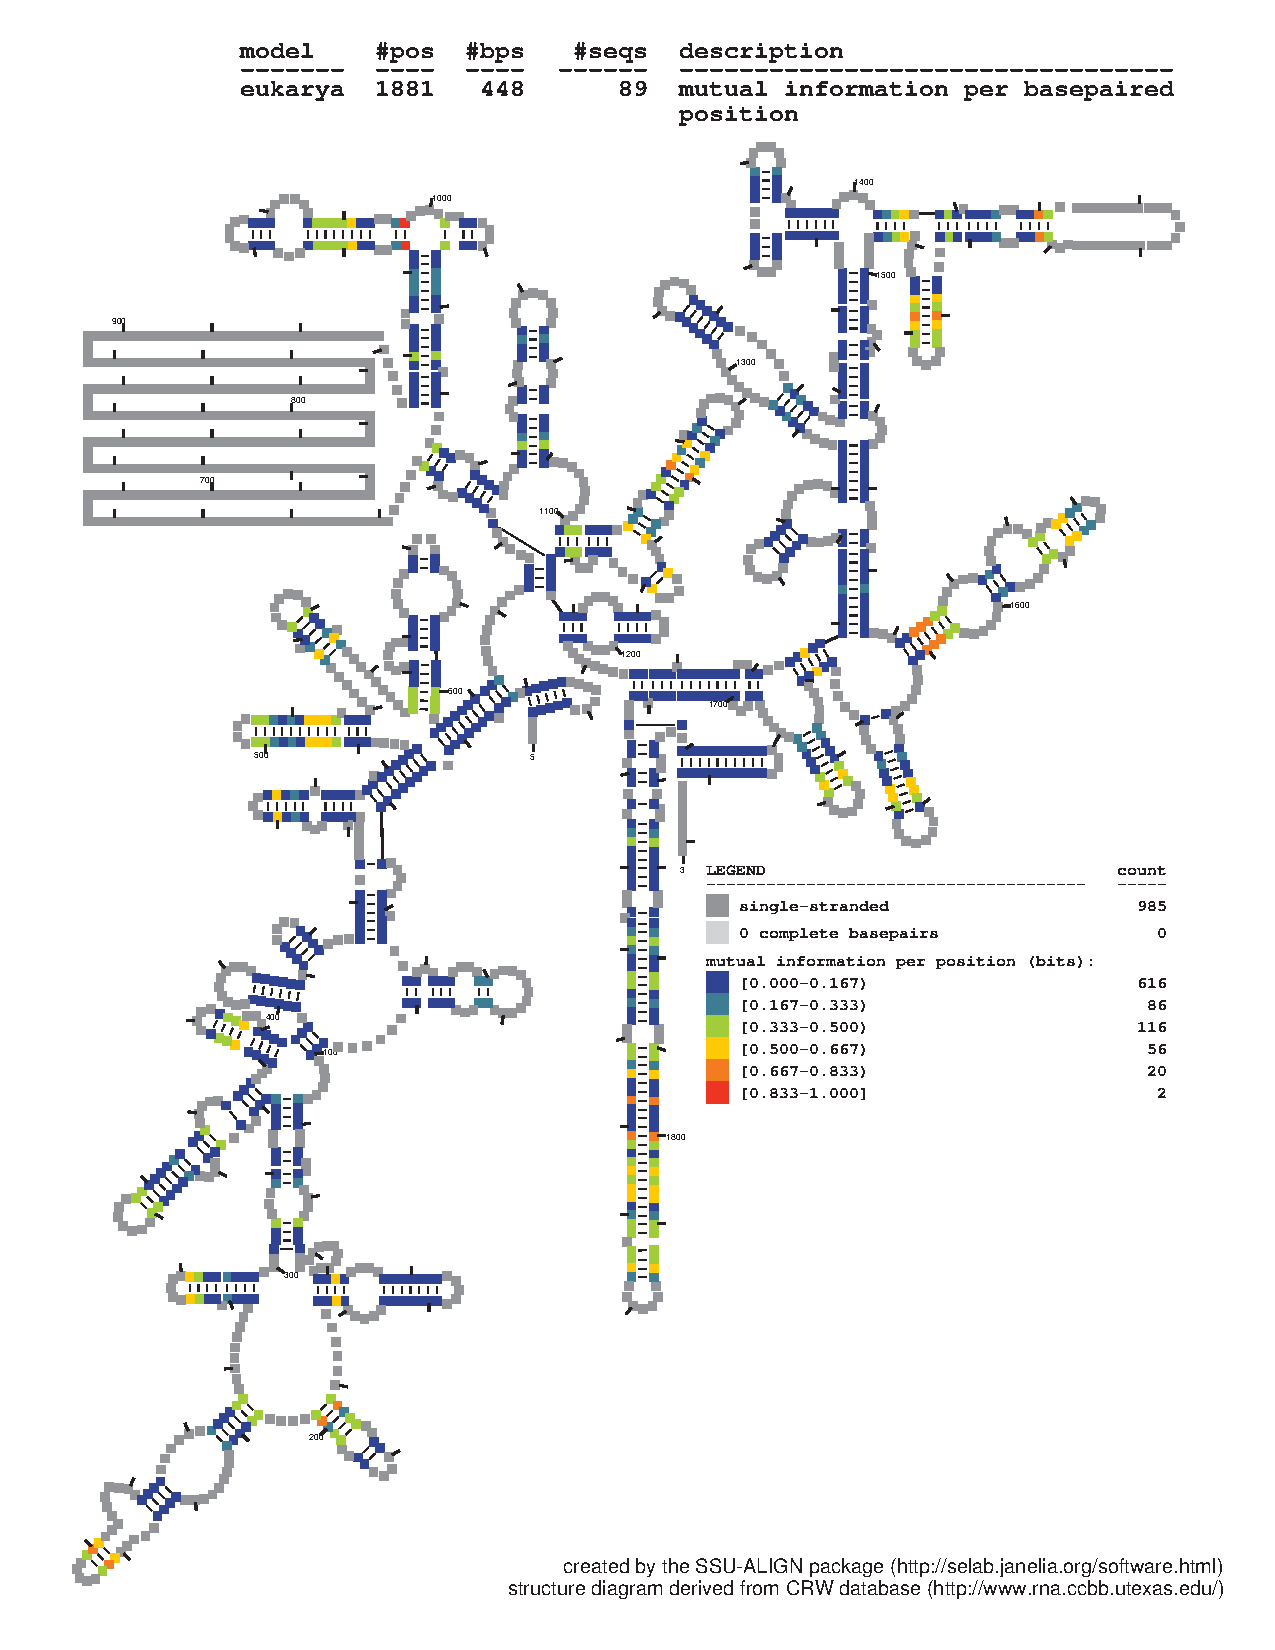
\includegraphics[width=5.7in]{Figures/eukarya-0p1-mutinfo}
\end{center}
\caption[Secondary structure diagram displaying extra information 
  from conserved structure per consensus position of the eukaryotic SSU seed
  alignment]{\textbf{Secondary structure diagram displaying extra
  information from conserved structure per consensus position of the eukaryotic SSU seed
  alignment.} Statistics correspond to the \sft{ssu-align} seed
  alignment derived from the \db{crw} database \cite{CannoneGutell02}
  as described in the text. This diagram was generated by the {\tt
  esl-ssudraw} program included in \sft{ssu-align}.}
\label{fig:euksinfo}
\end{figure}


\begin{figure}
\begin{center}
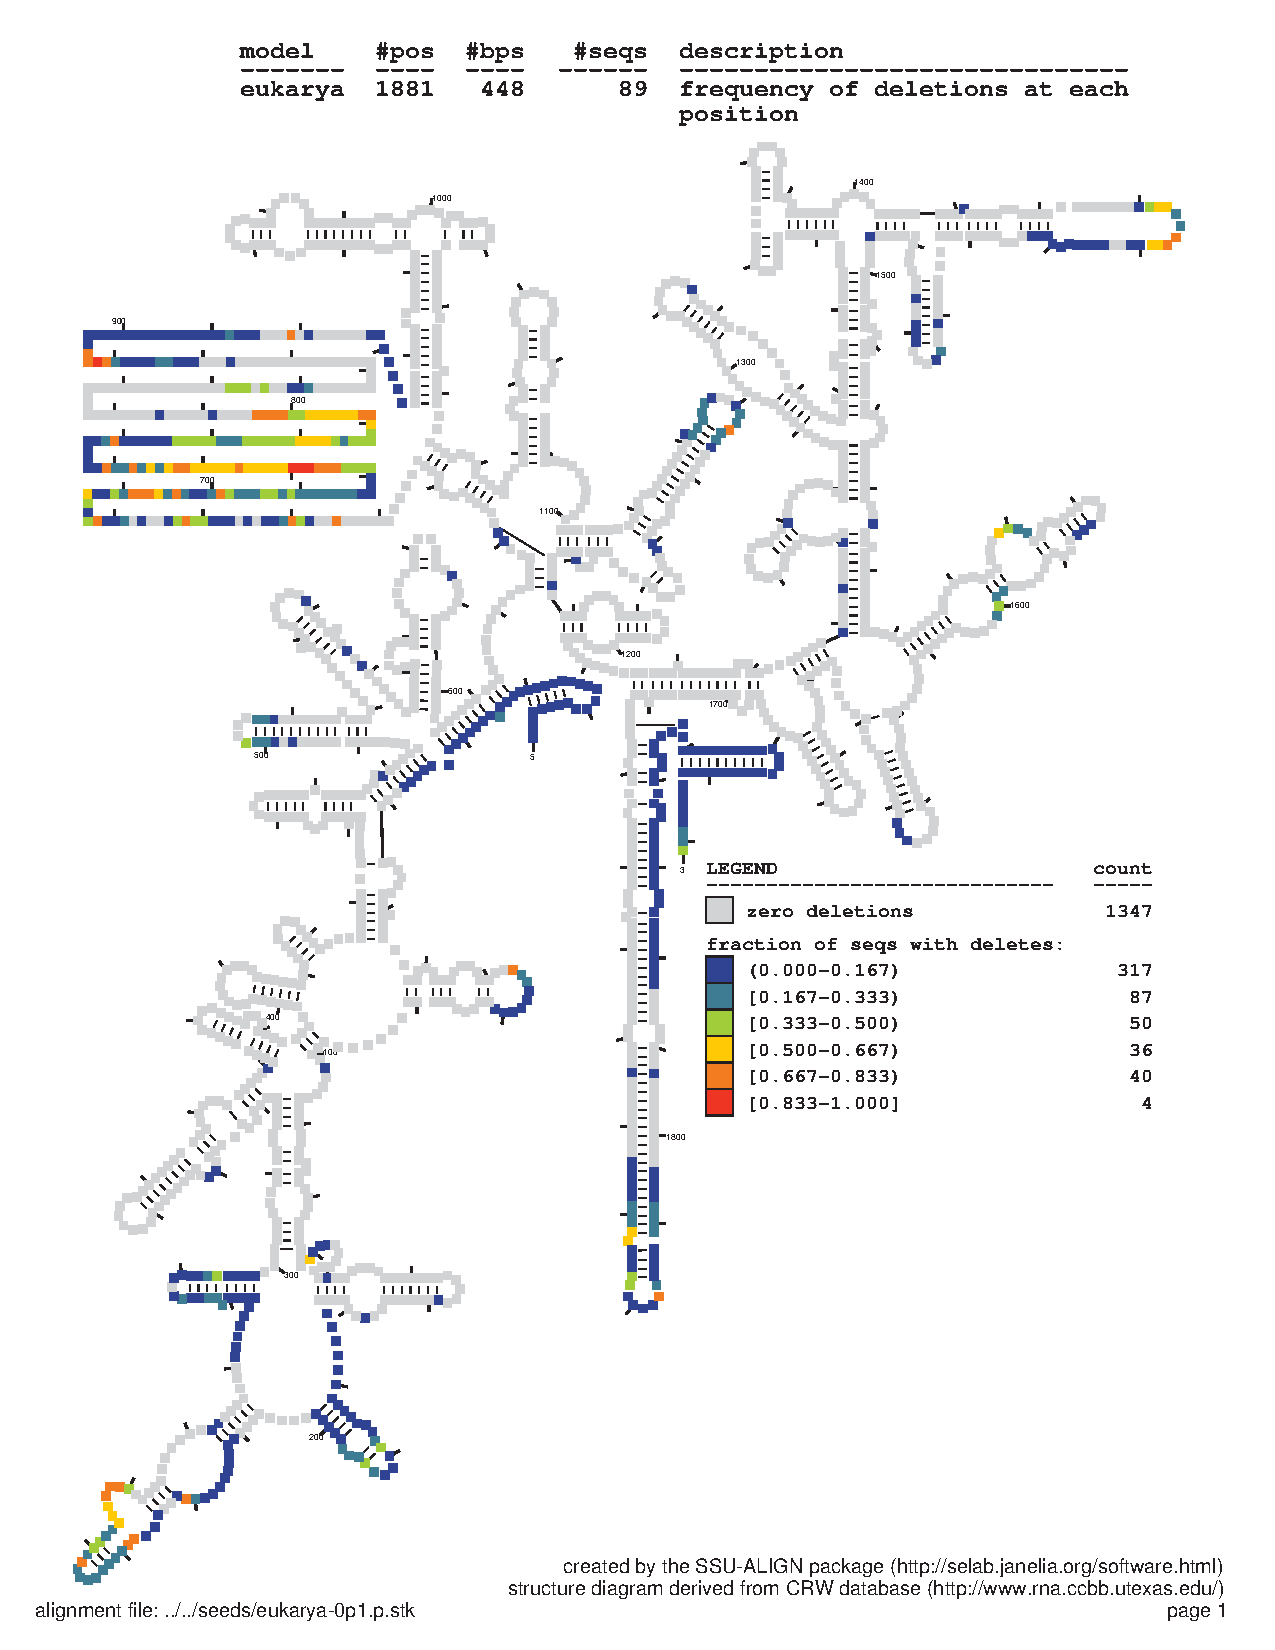
\includegraphics[width=5.7in]{Figures/eukarya-0p1-dall}
\end{center}
\caption[Secondary structure diagram displaying frequency of deletions
  per consensus position of the eukaryotic SSU seed
  alignment]{\textbf{Secondary structure diagram displaying frequency 
  of deletions per consensus position of the eukaryotic SSU seed
  alignment.} Statistics correspond to the \sft{ssu-align} seed
  alignment derived from the \db{crw} database \cite{CannoneGutell02}
  as described in the text. This diagram was generated by the {\tt
  esl-ssudraw} program included in \sft{ssu-align}.}
\label{fig:eukdel}
\end{figure}


\begin{figure}
\begin{center}
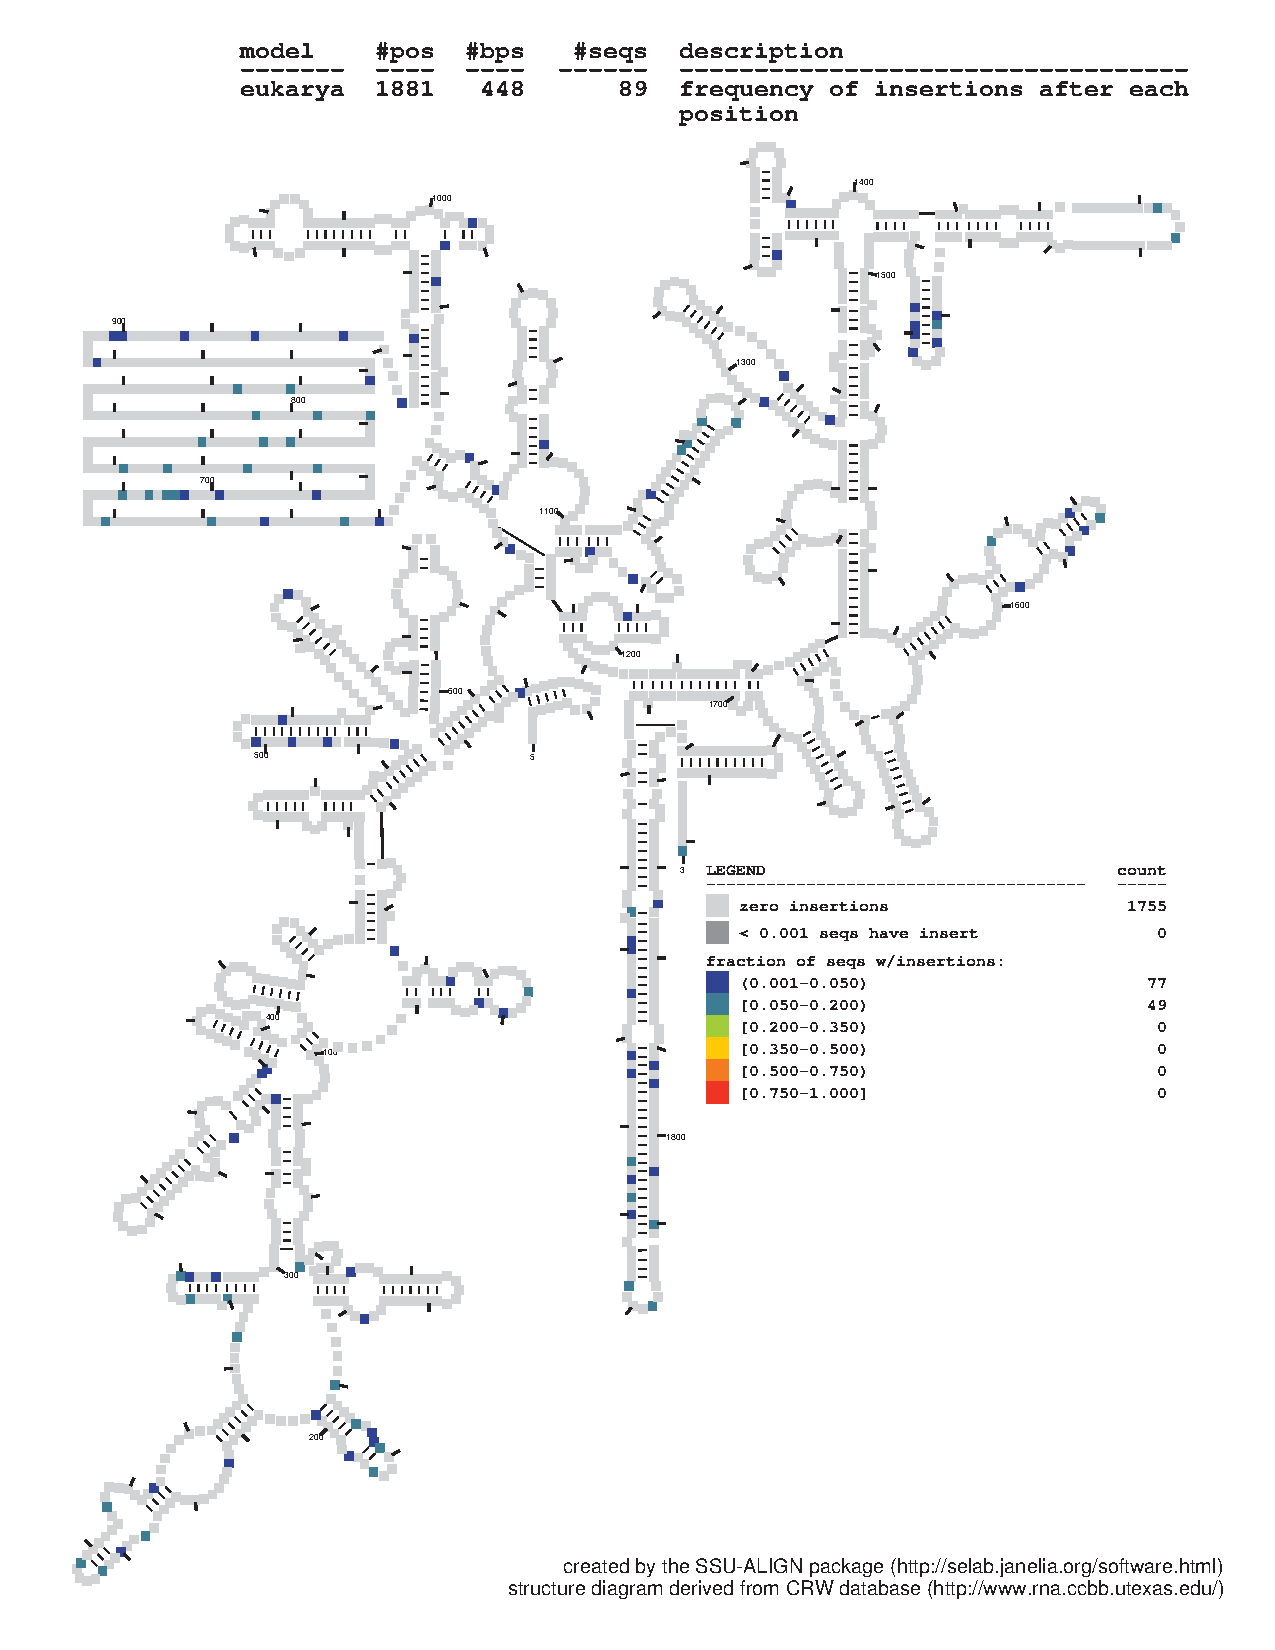
\includegraphics[width=5.7in]{Figures/eukarya-0p1-ifreq}
\end{center}
\caption[Secondary structure diagram displaying frequency of insertions
  after each consensus position in the eukaryotic SSU seed
  alignment]{\textbf{Secondary structure diagram displaying frequency
  of insertions after each consensus position in the eukaryotic SSU seed
  alignment.} Statistics correspond to the \sft{ssu-align} seed
  alignment derived from the \db{crw} database \cite{CannoneGutell02}
  as described in the text. This diagram was generated by the {\tt
  esl-ssudraw} program included in \sft{ssu-align}.}
\label{fig:eukins}
\end{figure}


